% This file makes a web version of the blueprint
% It should include all the \usepackage needed for this version.
% The template includes standard AMS packages.
% It is otherwise a very minimal preamble (you should probably at least
% add cleveref and tikz-cd).

\documentclass{report}

\usepackage{amssymb, amsthm, amsmath}
\usepackage{hyperref}
\usepackage{graphicx}
\usepackage[showmore, dep_graph]{blueprint}


% In this file you should put all LaTeX macros and settings to be used both by
% the pdf version and the web version.
% This should be most of your macros.

% The theorem-like environments defined below are those that appear by default
% in the dependency graph. See the README of leanblueprint if you need help to
% customize this.
% The configuration below use the theorem counter for all those environments
% (this is what the [theorem] arguments mean) and never resets it.
% If you want for instance to number them within chapters then you can add
% [chapter] at the end of the next line.
\newtheorem{theorem}{Theorem}
\newtheorem{proposition}[theorem]{Proposition}
\newtheorem{lemma}[theorem]{Lemma}
\newtheorem{corollary}[theorem]{Corollary}

\newtheorem{metatheorem}[theorem]{Metatheorem}
\newtheorem{metametatheorem}[theorem]{Meta-metatheorem}

\newtheorem{example}{Example}
\newtheorem{remark}{Remark}

\theoremstyle{definition}
\newtheorem{definition}[theorem]{Definition}
\numberwithin{theorem}{chapter}

\newcommand{\N}{\mathbb{N}}
\newcommand{\R}{\mathbb{R}}
\newcommand{\Z}{\mathbb{Z}}
\newcommand{\formaleq}{\simeq}
\newcommand{\op}{\diamond}

% This file makes a web version of the blueprint
% It should include all the \usepackage needed for this version.
% The template includes standard AMS packages.
% It is otherwise a very minimal preamble (you should probably at least
% add cleveref and tikz-cd).

\documentclass{report}

\usepackage{amssymb, amsthm, amsmath}
\usepackage{hyperref}
\usepackage[showmore, dep_graph]{blueprint}


% In this file you should put all LaTeX macros and settings to be used both by
% the pdf version and the web version.
% This should be most of your macros.

% The theorem-like environments defined below are those that appear by default
% in the dependency graph. See the README of leanblueprint if you need help to
% customize this.
% The configuration below use the theorem counter for all those environments
% (this is what the [theorem] arguments mean) and never resets it.
% If you want for instance to number them within chapters then you can add
% [chapter] at the end of the next line.
\newtheorem{theorem}{Theorem}
\newtheorem{proposition}[theorem]{Proposition}
\newtheorem{lemma}[theorem]{Lemma}
\newtheorem{corollary}[theorem]{Corollary}

\newtheorem{metatheorem}[theorem]{Metatheorem}
\newtheorem{metametatheorem}[theorem]{Meta-metatheorem}

\newtheorem{example}{Example}
\newtheorem{remark}{Remark}

\theoremstyle{definition}
\newtheorem{definition}[theorem]{Definition}
\numberwithin{theorem}{chapter}

\newcommand{\N}{\mathbb{N}}
\newcommand{\R}{\mathbb{R}}
\newcommand{\Z}{\mathbb{Z}}
\newcommand{\formaleq}{\simeq}
\newcommand{\op}{\diamond}

% This file makes a web version of the blueprint
% It should include all the \usepackage needed for this version.
% The template includes standard AMS packages.
% It is otherwise a very minimal preamble (you should probably at least
% add cleveref and tikz-cd).

\documentclass{report}

\usepackage{amssymb, amsthm, amsmath}
\usepackage{hyperref}
\usepackage[showmore, dep_graph]{blueprint}


% In this file you should put all LaTeX macros and settings to be used both by
% the pdf version and the web version.
% This should be most of your macros.

% The theorem-like environments defined below are those that appear by default
% in the dependency graph. See the README of leanblueprint if you need help to
% customize this.
% The configuration below use the theorem counter for all those environments
% (this is what the [theorem] arguments mean) and never resets it.
% If you want for instance to number them within chapters then you can add
% [chapter] at the end of the next line.
\newtheorem{theorem}{Theorem}
\newtheorem{proposition}[theorem]{Proposition}
\newtheorem{lemma}[theorem]{Lemma}
\newtheorem{corollary}[theorem]{Corollary}

\newtheorem{metatheorem}[theorem]{Metatheorem}
\newtheorem{metametatheorem}[theorem]{Meta-metatheorem}

\newtheorem{example}{Example}
\newtheorem{remark}{Remark}

\theoremstyle{definition}
\newtheorem{definition}[theorem]{Definition}
\numberwithin{theorem}{chapter}

\newcommand{\N}{\mathbb{N}}
\newcommand{\R}{\mathbb{R}}
\newcommand{\Z}{\mathbb{Z}}
\newcommand{\formaleq}{\simeq}
\newcommand{\op}{\diamond}

% This file makes a web version of the blueprint
% It should include all the \usepackage needed for this version.
% The template includes standard AMS packages.
% It is otherwise a very minimal preamble (you should probably at least
% add cleveref and tikz-cd).

\documentclass{report}

\usepackage{amssymb, amsthm, amsmath}
\usepackage{hyperref}
\usepackage[showmore, dep_graph]{blueprint}


\input{macros/common}
\input{macros/web}

\home{https://teorth.github.io/equational_theories}
\github{https://github.com/teorth/equational_theories}
\dochome{https://teorth.github.io/equational_theories/docs}

\title{Equational theories}
\author{Terence Tao}

\begin{document}
\maketitle
\input{content}
\end{document}

\home{https://teorth.github.io/equational_theories}
\github{https://github.com/teorth/equational_theories}
\dochome{https://teorth.github.io/equational_theories/docs}

\title{Equational theories}
\author{Terence Tao}

\begin{document}
\maketitle
% In this file you should put the actual content of the blueprint.
% It will be used both by the web and the print version.
% It should *not* include the \begin{document}
%
% If you want to split the blueprint content into several files then
% the current file can be a simple sequence of \input. Otherwise It
% can start with a \section or \chapter for instance.

\input{chapter/intro.tex}
\input{chapter/equations.tex}
\input{chapter/general_implications.tex}
\input{chapter/implications.tex}
\input{chapter/counterexamples.tex}
\input{chapter/constant.tex}
\input{chapter/metatheorems_from_invariants.tex}
\input{chapter/simple_rewrites.tex}
\input{chapter/trivial_auto.tex}
\input{chapter/all_small_magmas.tex}
\input{chapter/equation_search.tex}
\input{chapter/egraphs.tex}

\bibliographystyle{plain} % We choose the "plain" reference style
\bibliography{references}

\end{document}

\home{https://teorth.github.io/equational_theories}
\github{https://github.com/teorth/equational_theories}
\dochome{https://teorth.github.io/equational_theories/docs}

\title{Equational theories}
\author{Terence Tao}

\begin{document}
\maketitle
% In this file you should put the actual content of the blueprint.
% It will be used both by the web and the print version.
% It should *not* include the \begin{document}
%
% If you want to split the blueprint content into several files then
% the current file can be a simple sequence of \input. Otherwise It
% can start with a \section or \chapter for instance.

\chapter{Basic theory of magmas}

\begin{definition}[Magma]\label{magma-def}\lean{Magma}\leanok A \emph{magma} is a set $G$ equipped with a binary operation $\circ: G \times G \to G$.  A \emph{homomorphism} $\varphi : G \to H$ between two magmas is a map such that $\varphi(x \circ y) = \varphi(x) \circ \varphi(y)$ for all $x,y \in G$.  An \emph{isomorphism} is an invertible homomorphism.
\end{definition}

Groups, semi-groups, and monoids are familiar examples of magmas.  However, in general we do not expect magmas to have any associative properties.

A magma is called \emph{empty} if it has cardinality zero, \emph{singleton} if it has cardinality one, and \emph{non-trivial} otherwise.

The number of magma structures on a set $G$ of cardinality $n$ is of course $n^{n^2}$, which is \footnote{All sequences start from $n=0$ unless otherwise specified.}
$$ 1, 1, 16, 19683, 4294967296, 298023223876953125, \dots$$
(\href{https://oeis.org/A002489}{OEIS A002489}).
Up to isomorphism, the number of finite magmas of cardinality $n$ up to isomorphism is the slightly slower growing sequence
$$ 1, 1, 10, 3330, 178981952, 2483527537094825, 14325590003318891522275680, \dots$$
(\href{https://oeis.org/A001329}{OEIS A001329}).

\begin{definition}[Free Magma]\label{free-magma-def}\lean{FreeMagma}\leanok\uses{magma-def} The \emph{free magma} $M_X$ generated by a set $X$ (which we call an \emph{alphabet}) is the set of all finite formal expressions built from elements of $X$ and the operation $\circ$.  An element of $M_X$ will be called a \emph{word} with alphabet $X$.  The \emph{order} of a word is the number of $\circ$ symbols needed to generate the word.  Thus for instance $X$ is precisely the set of words of order $0$ in $M_X$.
\end{definition}

For sake of concreteness, we will take the alphabet $X$ to default to the natural numbers $\N$ if not otherwise specified.

For instance, if $X = \{0,1\}$, then $M_X$ would consist of the following words:
\begin{itemize}
  \item $0$, $1$ (the words of order $0$);
  \item $0 \circ 0$, $0 \circ 1$, $1 \circ 0$, $1 \circ 1$ (the words of order $1$);
  \item $0 \circ (0 \circ 0)$, $0 \circ (0 \circ 1)$, $0 \circ (1 \circ 0)$, $0 \circ (1 \circ 1)$, $1 \circ (0 \circ 0)$, $1 \circ (0 \circ 1)$, $1 \circ (1 \circ 0)$, $1 \circ (1 \circ 1)$, $(0 \circ 0) \circ 0$, $(0 \circ 0) \circ 1$, $(0 \circ 1) \circ 0$, $(0 \circ 1) \circ 1$, $(1 \circ 0) \circ 0$, $(1 \circ 0) \circ 1$, $(1 \circ 1) \circ 0$, $(1 \circ 1) \circ 1$ (the words of order $2$);
  \item etc.
\end{itemize}

\begin{lemma} \leanok \lean{FreeMagma.elementsOfNumNodesEq_card_eq_catalan_mul_pow} For a finite alphabet $X$, the number of words of order $n$ is $C_n |X|^{n+1}$, where $C_n$ is the $n^{\mathrm{th}}$ Catalan number and $X$ is the cardinality of $X$.
\end{lemma}

\begin{proof} \leanok Follows from standard properties of Catalan numbers.
\end{proof}

The first few Catalan numbers are
$$ 1, 1, 2, 5, 14, 42, 132, \dots$$
(\href{https://oeis.org/A000108}{OEIS A000108}).


\begin{definition}[Induced homomorphism]\label{induced-def}\uses{free-magma-def}  Given a function $f: X \to G$ from an alphabet $X$ to a magma $G$, the \emph{induced homomorphism} $\varphi_f: M_X \to G$ is the unique extension of $f$ to a magma homomorphism.  Similarly, if $\pi \colon X \to Y$ is a function, we write $\pi_* \colon M_X \to M_Y$ for the unique extension of $\pi$ to a magma homomorphism.
\end{definition}

For instance, if $f : \{0,1\} \to G$ maps $0,1$ to $x,y$ respectively, then
$$ \varphi_f(0 \circ 1) = x \circ y$$
$$ \varphi_f(1 \circ (0 \circ 1)) = y \circ (x \circ y)$$
and so forth.  If $\pi \colon \N \to \N$ is the map $\pi(n) := n+1$, then
$$ \pi_*(0 \circ 1) = 1 \circ 2$$
$$ \pi_*(1 \circ (0 \circ 1)) = 2 \circ (1 \circ 2)$$
and so forth.

\begin{definition}[Law]\label{law-def}\uses{induced-def}\lean{MagmaLaw}  Let $X$ be a set. A \emph{law} with alphabet $X$ is a formal expression of the form $w \formaleq w'$, where $w, w' \in M_X$ are words with alphabet $X$ (thus one can identify laws with alphabet $X$ with elements of $M_X \times M_X$).  A magma $G$ \emph{satisfies}\lean{satisfies} the law $w \formaleq w'$ if we have $\varphi_f( w ) = \varphi_f ( w' )$ for all $f: X \to G$, in which case we write $G \models w \formaleq w'$.
\end{definition}

Thus, for instance, the commutative law
\begin{equation}\label{comm-law}
  0 \circ 1 \formaleq 1 \circ 0
\end{equation}
is satisfied by a magma $G$ if and only if
\begin{equation}\label{comm-law-2}
 x \circ y = y \circ x
\end{equation}
for all $x, y \in G$.  We refer to \eqref{comm-law-2} as the \emph{equation} associated to the law \eqref{comm-law}.  One can think of equations as the ``semantic'' intrepretation of a ``syntactic'' law.  However, we shall often abuse notation and a law with its associated equation thus we shall (somewhat carelessly) also refer to \eqref{comm-law-2} as ``the commutative law'' (rather than ``the commutative equation'').

\begin{lemma}[Pushforward]\label{push}\uses{law-def}  Let $w \formaleq w'$ be a law with some alphabet $X$, $G$ be a magma, and $\pi: X \to Y$ be a function.  If $G \models w \formaleq w'$, then $G \models \pi_*(w) \formaleq \pi_*(w')$.  In particular, if $\pi$ is a bijection, the statements If $G \models w \formaleq w'$, then $G \models \pi_*(w) \formaleq \pi_*(w')$ are equivalent.
\end{lemma}

If $\pi$ is a bijection, we will call $\pi_*(w) \formaleq \pi_*(w')$ a \emph{relabeling} of the law $w \formaleq w'$.  Thus for instance
$$ 5 \circ 7 \formaleq 7 \circ 5$$
is a relabeling of the commutative law \eqref{comm-law}.  By the above lemma, relabeling does not affect whether a given magna satisfies a given law.

\begin{proof}  Trivial.
\end{proof}

\begin{lemma}[Equivalence]\label{equiv}\uses{law-def}  Let $G$ be a magma and $X$ be an alphabet.  Then the relation $G \models w \formaleq w'$ is an equivalence relation on $M_X$.
\end{lemma}

\begin{proof}  Trivial.
\end{proof}

Define the total order of a law $w \formaleq w'$ to be the sum of the orders of $w$ and $w'$.

\begin{lemma}[Counting laws up to relabeling]\label{law-count}\uses{push}  Up to relabeling, the number of laws $w \formaleq w'$ of total order $n$ is $C_{n+1} B_{n+2}$.
\end{lemma}

\begin{proof} Follows from the properties of Catalan and Bell numbers.
\end{proof}

The first few Bell numbers are
$$ 1, 1, 2, 5, 15, 52, 203, \dots$$
(\href{https://oeis.org/A000110}{OEIS A000110}).

The sequence in Lemma \ref{law-count} is
$$ 2, 10, 75, 728, 8526, 115764, \dots$$
(\href{https://oeis.org/A289679}{OEIS A289679}).

Now we would also like to count laws up to relabeling and symmetry.

\begin{lemma}[Counting laws up to relabeling and symmetry]\label{law-count-sym}\uses{push} Up to relabeling and symmetry, the number of laws $w \formaleq w'$ of total order $n$ is
$$ C_{n+1} B_{n+2}/2$$
when $n$ is odd, and
$$ (C_{n+1} B_{n+2} + C_{n/2} (2D_{n+2} - B_{n+2}))/2$$
when $n$ is even, where $D_n$ is the number of partitions of $[n]$ up to reflection.
\end{lemma}

\begin{proof} Elementary counting.
\end{proof}

The sequence $D_n$ is
$$ 1, 1, 2, 4, 11, 32, 117, \dots$$
(\href{https://oeis.org/A103293}{OEIS A103293}), and the sequence in Lemma \ref{law-count-sym} is
$$ 2, 5, 41, 364, 4294, 57882, 888440, \dots$$

We can also identify all laws of the form $w \formaleq w$ with the trivial law $0 \formaleq 0$.  The number of such laws of total order $n$ is zero if $n$ is odd, and $C_{n/2} B_{n/2+1}$ if $n$ is even.  We conclude:

\begin{lemma}[Counting laws up to relabeling, symmetry, and triviality]  Up to relabeling, symmetry, and triviality, the number of laws of total order $n$ is
$$ C_{n+1} B_{n+2}/2$$
if $n$ is odd, $2$ if $n = 0$, and
$$ (C_{n+1} B_{n+2} + C_{n/2} (2D_{n+2} - B_{n+2}))/2 - C_{n/2} B_{n/2+1}$$
if $n \geq 2$ is even.
\end{lemma}

\begin{proof} Routine counting.
\end{proof}

This sequence is
$$2, 5, 39, 364, 4284, 57882, 888365, \dots$$

In particular, up to relabeling, symmetry, and triviality, there are exactly $4694$ laws of total order at most $4$.  A list can be found \href{https://github.com/teorth/equational_theories/blob/main/data/equations.txt}{here}.  A script for generating them may be found \href{https://github.com/teorth/equational_theories/blob/main/scripts/generate_eqs_list.py}{here}.  The list is sorted by the total number of operations, then by the number of operations on the LHS. Within each such class we define an order on expressions by variable $<$ operation, and lexical order on variables.

\chapter{Equations}

\begin{definition}[Equation 1]\label{eq1}\lean{Equation1}\leanok\uses{magma-def}  Equation 1 is the law $x=x$.
\end{definition}

\begin{definition}[Equation 2]\label{eq2}\lean{Equation2}\leanok\uses{magma-def}  Equation 2 is the law $x=y$.
\end{definition}

\begin{definition}[Equation 3]\label{eq3}\lean{Equation3}\leanok\uses{magma-def}  Equation 3 is the law $x=x \circ x$.
\end{definition}

\begin{definition}[Equation 4]\label{eq4}\lean{Equation4}\leanok\uses{magma-def}  Equation 4 is the law $x=x \circ y$.
\end{definition}

\begin{definition}[Equation 5]\label{eq5}\lean{Equation5}\leanok\uses{magma-def}  Equation 5 is the law $x=y \circ x$.
\end{definition}

\begin{definition}[Equation 6]\label{eq6}\lean{Equation6}\leanok\uses{magma-def}  Equation 6 is the law $x=y \circ y$.
\end{definition}

\begin{definition}[Equation 7]\label{eq7}\lean{Equation7}\leanok\uses{magma-def}  Equation 7 is the law $x=y \circ z$.
\end{definition}

\begin{definition}[Equation 8]\label{eq8}\lean{Equation8}\leanok\uses{magma-def}  Equation 8 is the law $x=x \circ (x \circ x)$.
\end{definition}

\begin{definition}[Equation 42]\label{eq42}\lean{Equation42}\leanok\uses{magma-def}  Equation 42 is the law $x \circ y = x \circ z$.
\end{definition}

\begin{definition}[Equation 43]\label{eq43}\lean{Equation43}\leanok\uses{magma-def}  Equation 43 is the law $x \circ y = y \circ x$.
\end{definition}

\begin{definition}[Equation 46]\label{eq46}\lean{Equation46}\leanok\uses{magma-def}  Equation 46 is the law $x \circ y = z \circ w$.
\end{definition}

\begin{definition}[Equation 168]\label{eq168}\lean{Equation168}\leanok\uses{magma-def}  Equation 168 is the law $x = (y \circ x) \circ (x \circ z)$.
\end{definition}

\begin{definition}[Equation 387]\label{eq387}\lean{Equation387}\leanok\uses{magma-def}  Equation 387 is the law $x \circ y = (y \circ y) \circ x$.
\end{definition}

\begin{definition}[Equation 4512]\label{eq4512}\lean{Equation4512}\leanok\uses{magma-def}  Equation 4512 is the law $x \circ (y \circ z) = (x \circ y) \circ z$.
\end{definition}

\begin{definition}[Equation 4513]\label{eq4513}\lean{Equation4513}\leanok\uses{magma-def}  Equation 4513 is the law $x \circ (y \circ z) = (x \circ y) \circ w$.
\end{definition}

\begin{definition}[Equation 4552]\label{eq4552}\lean{Equation4552}\leanok\uses{magma-def}  Equation 4552 is the law $x \circ (y \circ z) = (x \circ w) \circ u$.
\end{definition}

\begin{definition}[Equation 4582]\label{eq4582}\lean{Equation4582}\leanok\uses{magma-def}  Equation 4582 is the law $x \circ (y \circ z) = (w \circ u) \circ v$.
\end{definition}

\chapter{General implications}

We will be interested in seeing which laws imply which other laws, in the sense that magmas obeying the former law automatically obey the latter.  We will also be interested in \emph{anti-implications} showing that one law does \emph{not} imply another, by producing examples of magmas that obey the former law but not the latter. Here is a formal definition.

\begin{definition}[Implication]\label{impl}\uses{law-def}  A law $w  \formaleq  w'$ is said to \emph{imply} another law $w''  \formaleq  w'''$, if every magma $G$ that satisfies the former, satisfies the latter:
  $$ G \models w  \formaleq  w' \implies G \models w''  \formaleq  w'''.$$
Two laws are said to be \emph{equivalent} if they imply each other.
\end{definition}

\begin{lemma}[Pre-order]\label{pre-order}\uses{impl}  Implication is a pre-order on the set of laws, and equivalence is an equivalence relation.
\end{lemma}

\begin{proof} Trivial.
\end{proof}

Implications between the laws from Chapter \ref{subgraph-eq} are depicted in Figure \ref{fig:implications}.

\begin{figure}
  \centering
  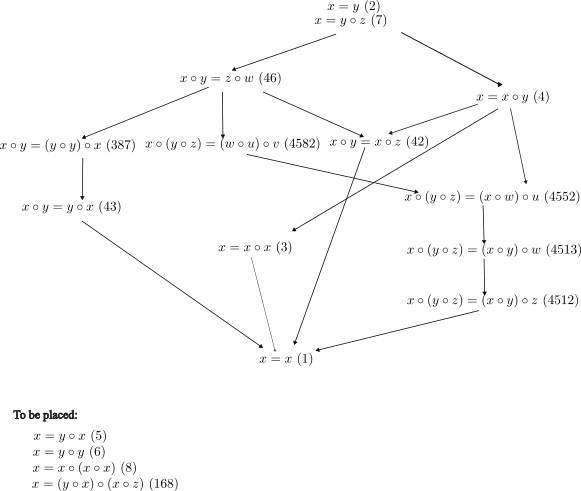
\includegraphics[width=0.5\linewidth]{../../images/implications.png}
  \caption{Implications between the above equations, displayed as a Hasse diagram.}
  \label{fig:implications}
\end{figure}


\begin{lemma}[Minimal element]\label{minimal}\uses{pre-order}  The law $0  \formaleq  0$ is the minimal element in this pre-order.
\end{lemma}

\begin{proof} Trivial.
\end{proof}

\begin{lemma}[Maximal element]\label{maximal}\uses{pre-order}  The law $0  \formaleq  0$ is the minimal element in this pre-order.
\end{lemma}

\begin{proof} Trivial.
\end{proof}

Every magma $G$ has a \emph{reversal} $G^{\mathrm{op}}$, formed by by replacing the magma operation $\circ$ with its opposite $\circ^{\mathrm{op}}:(x,y) \mapsto y \circ x$. There is a natural isomorphism between these magmas, which induces an involution $w \mapsto w^{\mathrm{op}}$ on words $w \in M_X$.  Every law $w  \formaleq  w'$ then has a \emph{dual} $w^{\mathrm{op}}  \formaleq  (w')^{\mathrm{op}}$.

For instance, the dual of the law $0 \circ 1 = 0 \circ 2$ is $1 \circ 0 = 2 \circ 0$, which after relabeling is $0 \circ 1 = 2 \circ 1$.  A list of equations and their duals can be found \href{https://github.com/teorth/equational_theories/blob/main/data/dual_equations.md}{here}.  Of the 4694 equations under consideration, 84 are self-dual, leaving 2305 pairs of dual equations.

The pre-ordering on laws has a duality symmetry:

\begin{lemma}[Duality of laws]\label{duality}\uses{pre-order}  If $w  \formaleq  w'$ implies $w''  \formaleq  w'''$, then $w^{\mathrm{op}}  \formaleq  (w')^{\mathrm{op}}$ implies $w''^{\mathrm{op}}  \formaleq  (w''')^{\mathrm{op}}$.
\end{lemma}

\begin{proof} This follows from the fact that a magma $G$ satisfies a law $w  \formaleq  w'$ if and only if $G^{\mathrm{op}}$ satisfies $w^{\mathrm{op}}  \formaleq  (w')^{\mathrm{op}}$.
\end{proof}

Some equational laws can be ``diagonalized'':

\begin{theorem}[Diagonalization]\label{diag}  An equational law of the form
  \begin{equation}\label{prediag} F(x_1,\dots,x_n) = G(y_1,\dots,y_m),
  \end{equation}
  where $x_1,\dots,x_n$ and $y_1,\dots,y_m$ are distinct elements of the alphabet, implies the diagonalized law
$$ F(x_1,\dots,x_n) = F(x'_1,\dots,x'_n).$$
where $x'_1,\dots,x'_n$ are distinct from $x_1,\dots,x_n$
In particular, if $G(y_1,\dots,y_m)$ can be viewed as a specialization of $F(x'_1,\dots,x'_n)$, then these two laws are equivalent.
\end{theorem}

\begin{proof}  From two applications of \eqref{prediag} one has
$$ F(x_1,\dots,x_n) = G(y_1,\dots,y_m)$$
and
$$ F(x'_1,\dots,x'_n) = G(y_1,\dots,y_m)$$
whence the claim.
\end{proof}

Thus for instance, Definition \ref{eq7} is equivalent to Definition \ref{eq2}.

\begin{theorem}[Laws implied by the constant law]\label{constant-impl}\uses{impl,eq46}  If $w, w'$ each have order at least one, then the law $w \formaleq w'$ is implied by the constant law (Definition \ref{eq46}).  If exactly one of $w, w'$ has order zero, and the law $w \formaleq w'$ is not implied by the constant law.
\end{theorem}

\begin{proof} Routine.
\end{proof}

\begin{theorem}[Criterion for implication]\label{variable-impl}\uses{impl}  If $w \formaleq w'$ is such that every variable appears the same number of times in both $w$ and $w'$, and $w \formaleq w'$ implies another law $w'' \formaleq w'''$, then every variable appears the same number of times in both $w''$ and $w'''$.
\end{theorem}

\begin{proof} Consider the magma $\R$ with the addition law $+$.  By hypothesis, this magma obeys $w \formaleq w'$, and hence $w'' \formaleq w'''$, giving the claim by comparing coefficients of the linear forms associated to $w''$ and $w'''$ in this magma.
\end{proof}

\chapter{Implications between selected laws}

We collect here some notable implications between the the selected laws in Chapter \ref{subgraph-eq}.   By Theorem \ref{sound-complete}, every implication can basically be established by a finite number of rewrites.  In most cases, the sequence of rewrites is quite straightforward, and the implication is very easy, but we record some less obvious examples.

\begin{theorem}[387 implies 43]\label{387_implies_43}\uses{eq387,eq43}\lean{Subgraph.Equation387_implies_Equation43}\leanok  Definition \ref{eq387} implies Definition \ref{eq43}.
\end{theorem}

\begin{proof}\leanok (From \href{https://mathoverflow.net/a/450905/766}{MathOverflow}).
  By Definition \ref{eq387}, one has the law
\begin{equation}\label{387-again}
  (x \op x) \op y = y \op x.
\end{equation}
Specializing to $y=x \op x$, we conclude
$$(x \op x) \op (x \op x) = (x \op x) \op x$$
and hence by another application of \eqref{eq387} we see that $x \op x$ is idempotent:
\begin{equation}\label{idem}
  (x \op x) \op (x \op x) = x \op x.
\end{equation}
Now, replacing $x$ by $x \op x$ in \eqref{387-again} and then using \eqref{idem} we see that
$$ (x \op x) \op y = y \op (x \op x)$$
so in particular $x \op x$ commutes with $y \op y$:
\begin{equation}\label{op-idem} (x \op x) \op (y \op y) = (y \op y) \op (x \op x).
\end{equation}
Also, from two applications of \eqref{387-again} one has
$$(x \op x) \op (y \op y) = (y \op y) \op x = x \op y.$$
Thus \eqref{op-idem} simplifies to $x \op y = y \op x$, which is Definition \ref{eq43}.
\end{proof}

\begin{theorem}[29 equivalent to 14]\label{29_equiv_14} \uses{eq29,eq14}\lean{Subgraph.Equation29_implies_Equation14}\leanok  Definition \ref{eq29} is equivalent to Definition \ref{eq14}.
\end{theorem}

This result was posed as Problem A1 from Putnam 2001.

\begin{proof}\leanok\uses{duality} By Lemma \ref{duality} it suffices to show that Definition \ref{eq29} implies Definition \ref{eq14}.  From Definition \ref{eq29} one has
  $$ x = ((x \op y) \op x) \op (x \op y)$$
  and also
  $$ y = (x \op y) \op x$$
  giving $x = y \op (x \op y)$, which is Definition \ref{eq14}.
\end{proof}

\begin{theorem}[14 implies 29]\label{14_implies_29} \uses{eq29,eq14}\lean{Subgraph.Equation14_implies_Equation29}\leanok  Definition \ref{eq14} implies Definition \ref{eq29}.
\end{theorem}

This result was posed as Problem A1 from Putnam 2001.

\begin{proof}\leanok
\end{proof}

The following result was Problem A4 on Putnam 1978.

\begin{theorem}[3744 implies 3722, 381]\label{3744_implies_3722_381}\uses{eq3744, eq3722, eq381}\lean{Subgraph.Equation3744_implies_Equation3722, Subgraph.Equation3744_implies_Equation381}\leanok Definition \ref{eq3744} implies Definition \ref{eq3722} and Definition \ref{eq381}.
\end{theorem}

\begin{proof}\leanok By hypothesis, one has
$$x \op y = (x \op z) \op (w \op y)
  $$
for all $x,y,z,w$.  Various specializations of this give
\begin{align}
 x \op y &= (x \op z) \op (y \op y) \label{381-1} \\
 x \op z &= (x \op z) \op (x \op z) \label{381-2} \\
(x \op z) \op y &= ((x \op z) \op (x \op z)) \op (y \op y) \label{381-3}.
\end{align}
The equation \eqref{381-2} gives Definition \ref{eq3722}, while \eqref{381-1}, \eqref{381-2}, \eqref{381-3} gives
$$ x \op y = (x\op z) \op y$$
which is Definition \ref{eq381}.
\end{proof}

\begin{theorem}[1689 is equivalent to 2]\label{1689_equiv_2}\uses{eq1689, eq2}\lean{Subgraph.Equation1689_implies_Equation2, Subgraph.Equation2_implies_Equation1689}\leanok Definition \ref{eq1689} is equivalent to Definition \ref{eq2}.
\end{theorem}


\begin{proof}\leanok  The implication of Definition \ref{eq1689} from Definition \ref{eq2} is trivial.  The converse is a surprisingly long chain of implications; see pages 326--327 of \cite{Kisielewicz2}.  The initial law
$$ x = (y \op x) \op ((x \op z) \op z)$$
is used to obtain, in turn,
$$ x \op ((((x \op y) \op y) \op z) \op z) = (x \op y) \op y,$$
$$(x \op (y \op z)) \op (z \op ((z \op w) \op w)) = y \op z,$$
$$x \op (y \op ((y \op z) \op z)) = (x \op y) \op y,$$
$$((x \op (y \op z)) \op z) \op z = y \op z,$$
$$(x \op (y \op (z \op w))) \op (z \op w) = y \op (z \op w),$$
$$(x \op (y \op z)) \op (y \op z) = x \op (y \op z),$$
$$((x \op y) \op ((y \op z) \op z)) \op ((y \op z) \op z) = y,$$
$$((x \op y) \op ((y \op z) \op z)) \op ((y \op z) \op z) = ((x \op ((x \op y) \op ((y \op z) \op z))) \op ((y \op z) \op z)) \op ((y \op z) \op z),$$
$$ x \op ((x \op y) \op y) = x,$$
$$ x \op (x \op (y \op z)) = x,$$
$$ (x \op y) \op y = x \op y,$$
$$ (x \op x) \op x = x,$$
$$ (x \op y) \op y = y,$$
$$ x \op y = y.$$
\end{proof}

The following result was established in \cite{mendelsohn-padmanabhan}.

\begin{theorem}[Consequences of 1571]\label{1571_impl}\uses{eq1571, eq2662, eq40, eq23, eq8, eq16, eq14, eq43, eq4512}\lean{Subgraph.Equation1571_implies_Equation2662, Subgraph.Equation1571_implies_Equation40, Subgraph.Equation1571_implies_Equation23,Subgraph.Equation1571_implies_Equation8, Subgraph.Equation1571_implies_Equation16, Subgraph.Equation1571_implies_Equation43, Subgraph.Equation1571_implies_Equation4512}\leanok  Magmas obeying Definition \ref{eq1571} also obey Definitions \ref{eq2662}, \ref{eq40}, \ref{eq23}, \ref{eq8}, \ref{eq16}, \eqref{eq14}, \ref{eq43}, and \ref{eq4512}, and are in fact abelian groups of exponent two.  Conversely, all abelian groups of exponent two obey Definition \ref{eq1571}.
\end{theorem}

\begin{proof}\leanok  Suppose that a magma $G$ obeys Definition \ref{eq1571}, thus
\begin{equation}\label{1571-again}
 x = (y \op z) \op (y \op (x \op z)).
\end{equation}
$$ x = ((x \op y) \op (x \op y)) \op ((x \op y) \op (x \op (x \op y)))$$
and
$$ x = (x \op y) \op (x \op (x \op y))$$
whence
$$x = ((x \op y) \op (x \op y)) \op x$$
which is Definition \ref{eq2662}.  This gives
$$y = ((y \op z) \op (y \op z)) \op y$$
while from \eqref{1571-again} one has
$$ (y \op z) \op (y \op z) = (x \op y) \op (x \op ((y \op z) \op (y \op z) \op y))$$
whence
$$ (x \op y) \op (x \op y) = (y \op z) \op (y \op z).$$
This implies that $(x \op y) \op (x \op y)$ does not depend on $x$, or on $y$, hence is equal to some constant $e$:
$$ (x \op y) \op (x \op y) = e.$$
From \eqref{1571-again} the magma operation is surjective, hence
\begin{equation}\label{xxe} x \op x = e
\end{equation}
which gives Definition \ref{eq40}.  Applying \eqref{1571-again} with $x=y=z$ we conclude
$$ x = e \op (x \op e)$$
while if we instead take $y=z=e$ we have
$$ x = e \op (e \op (x \op e))$$
hence
$$ x = e \op x$$
and then also
$$ x = x \op e$$
from which we readily conclude Definitions \ref{eq23}, \ref{eq8}; thus $e$ is an identity element.  From \eqref{1571-again} with $z=e$ we now have
\begin{equation}\label{16-again}
 x = y \op (y \op x)
\end{equation}
which is Definition \ref{eq16}. If instead we take $y=e$ we have
\begin{equation}\label{14-again}
  x = z \op (x \op z)
\end{equation}
which is Definition \ref{eq14}.  So if we substitute $z = x \op y$ and use \eqref{16-again} we obtain
$$ x = (x \op y) \op y$$
and hence
$$ y \op x = y \op ((x \op y) \op y) = x \op y$$
thanks to \eqref{14-again}.  This gives Definition \ref{eq43}, thus $G$ is now commutative.  From \eqref{1571-again} once more one has
$$x \op (y \op z) = (y \op x) \op (z \op ((x \op (y \op z)) \op x))$$
which one can simplify using commutativity and \eqref{16-again} (or \eqref{14-again}) to eventually obtain
$$x \op (y \op z) = (x \op y) \op z$$
which is Definition \ref{eq4512}.  $G$ is now commutative and associative, and every element is its own inverse and of exponent $2$, hence is an abelian group thanks to \eqref{xxe}, so $G$ is an abelian group of exponent $2$ as claimed.  The converse is easily verified.
\end{proof}

\begin{theorem}[953 is equivalent to 2]\label{953_equiv_2}\uses{eq953, eq2}\lean{Subgraph.Equation953_implies_Equation2}\leanok  Definition \ref{eq953} is equivalent to Definition \ref{eq2}.
\end{theorem}

\begin{proof}\leanok  It suffices to show that Definition \ref{eq953} implies Definition \ref{eq2}.  Pick an element $0$ of $G$ and define $1 = 0 \op 0$ and $2 = 1 \op 1$ (we do not require $0,1,2$ to be distinct).
From Definition \ref{eq953} with $x=z=0$ we have
$$ 0 = y \op 2.$$
If we then apply Definition \ref{eq953} with $z=1$ we conclude that
$$ x = y \op 0$$
for all $x,y$, from which one concludes $x=x'$ for any $x,x' \in G$, giving Definition \ref{eq2}.
\end{proof}


Some other notable equational laws are as follows.

\begin{theorem}[Sheffer stroke axiom]\label{sheffer}  The law
$$ 0 \formaleq (1 \op ((0 \op 1) \op 1)) \op (0 \op (2 \op 1))$$
or in equation form
$$ x = y \op ((x \op y) \op y) \op (x \op (z \op y)) $$
axiomatizes the Sheffer stroke operation. {\bf TODO: locate the equation number for this law.}
\end{theorem}

\begin{proof}
See \cite{mccune_et_al}.  In fact this is the shortest law with this property.
\end{proof}

A \emph{natural central groupoid} is, up to isomorphism, a magma with carrier $S \times S$ for some set $S$ and operation
$$ (a,b) \op (c,d) = (b,c).$$
These are examples of central groupoids (Definition \ref{eq168}).

\begin{theorem}[Natural central groupoid axiom]\label{natural-central-groupoid}  The law
$$ 0 \formaleq (1 \op ((2 \op 0) \op 3)) \op (0 \op 3)$$
or in equation form
\begin{equation}\label{26302}
  x = (y \op ((z \op x) \op w)) \op (x \op w)
\end{equation}
(Equation 26302) characterizes natural central groupoids.
\end{theorem}

\begin{proof}
  See \cite[Theorem 5]{knuth}.  The proof is quite lengthy; a sketch is as follows. It is easy to see that natural central groupoids obey \eqref{26302}.  Conversely, if this law holds, then
\begin{align*}
  (y \op z) \op (z \op w) &= (( x \op ((w \op (y \op z)) \op w)) \op ((y \op z) \op w)) \op (z \op w)\\
  &= z
\end{align*}
so we have a central groupoid.  Setting $y = (t \op t) \op t$, $z = t \op (t \op t)$, $w = t \op t$ in \eqref{26302} we also obtain
$$ (x \op t) \op t = (t \op t) \op t.$$
Using the notation
$$ x^{(1)} := (x \op x) \op x, \quad x^{(2)} := x \op (x \op x)$$
we then have
\begin{align*}
  x \op t &= ((x \op x) \op (x \op t)) \op ((x \op t) \op t) \\
  &= x \op t^{(1)}.
\end{align*}
A lengthy computer-assisted argument then gave the dual identity
$$ t^{(2)} \op x = t \op x$$
Together, these give
$$ x^{(2)} \op y^{(1)} = x \op y.$$
Multiplying on the left by $x = x^{(1)}\op x^{(2)}$, one can conclude that
$$ x^{(2)} = x \op (x \op y).$$
One then has
\begin{align*}
  (x \op y)^{(1)} &= ((y \op x) \op (x \op y)) \op (x \op y) \\
&= x \op (x \op y) \\
&= x^{(2)}
\end{align*}
and a similar argument gives
$$ (x \op y)^{(2)} = y^{(1)}.$$
Since $(x \op x)^{(1)} = x^{(2)}$ and $(x \op x)^{(2)} = x^{(1)}$, we conclude that $x^{(1)}$ and $x^{(2)}$ are idempotent.  Since $x = x^{(1)} \op x^{(2)}$, we see that every $x$ is the product of two idempotents.  One can show that this representation is unique, and gives a canonical identification with a natural central groupoid.
\end{proof}

\chapter{Selected magmas}

Each magma can be used to establish anti-implications: if $\Gamma$ is the set of all laws obeyed by a magma $G$, then we have $\not E \leq E'$ whenever $E \in \Gamma$ and $E' \not \in \Gamma$.  Large numbers of implications can already be obtained from

\begin{itemize}
  \item All magmas of order at most $4$, up to isomorphism (of which there are $178,985,294$);
  \item All commutative magmas of order $5$, up to isomorphism {\bf determine their count};
  \item Cyclic groups $\Z/N\Z$ with $2 \leq N \leq 12$ and $x \circ y = ax^2+bxy+cy^2+dx+ey$ for randomly chosen $a,b,c,d,e$.
  \item There are only $1410$ distinct cancellative magmas of order $5$ (up to isomorphism), and Mace4 can generate all of them in under 20 seconds. A shell script to do this is available \href{https://github.com/zaklogician/equational_theories/tree/cancellative_magmas/scripts/cancellative_magmas}{here}. A magma is cancellative if $xy=xz$ implies $y=z$ and $yx=zx$ implies $y=z$.
\end{itemize}


Some other magmas have been used to establish counterexamples:
\begin{itemize}
  \item The cyclic group $\Z/6\Z$ with the addition law.
  \item The natural numbers with law $x \circ y = x+1$.
  \item The natural numbers with law $x \circ y = xy+1$.
  \item The reals with $x \circ y = (x+y)/2$.
  \item The natural numbers with $x \circ x$ equal to $x$ when $x=y$ and $x+1$ otherwise.
\end{itemize}

\chapter{Equivalence with the constant and singleton laws}

\href{https://github.com/teorth/equational_theories/blob/main/equational_theories/Generated/Constant.lean}{85 laws}
have been shown to be equivalent to the constant law (Definition \ref{eq46}), and
\href{https://github.com/teorth/equational_theories/blob/main/equational_theories/Generated/Singleton.lean}{815 laws}
have been shown to be equivalent to the singleton law (Definition \ref{eq2}).

These are the laws up to 4 operations that follow from diagonalization of \ref{eq2} and \ref{eq46}.

To formalize these in Lean, a search was run on the list of equations to discover
diagonalizations of these two specific laws: equations of the form $x = R$ where $R$ doesn't include
$x$, and equations of the form $x \circ y = R$ where $R$ doesn't include $x$ or $y$.

The proofs themselves all look alike, and correspond exactly to the two steps described in the proof
of \ref{diag}. The Lean proofs were generated semi-manually, using search-and-replace starting from
the output of \texttt{grep} that found the diagonalized laws.

In the case of the constant law, equation \ref{eq41} ($x \circ x = y \circ z$) wasn't detected using
this method. It was added manually to the file with the existing proof from the sub-graph project.

\chapter{Metatheorems from Invariants}
For the purposes of this chapter, a \emph{theorem} is a (true) statement about particular equations, for example `(387 implies 43)' is a theorem. A \emph{metatheorem} is a general statement about implications; one can usually get many theorems from a single metatheorem. This chapter is all about generating many interesting metatheorems using a \emph{meta-metatheorem}, called the fundamental property of invariants. If all this is making your head spin, don't worry. Look at [REFERENCES] for examples of metatheorems you can probably agree are both concrete and interesting. Once you have done that, come back here and we will show you how to prove these and other metatheorems using \emph{invariants}.

\section{Invariants}
Let $E, E_1$, and $E_2$ be equations. If $E \Rightarrow E_1$ and $E_1 \Rightarrow E_2$, then $E \Rightarrow E_2$. Very trivial. Rephrasing this, we see that if $E \Rightarrow E_1$ and $E \nRightarrow E_2$, then $E_1\nRightarrow E_2$. 

Extending this idea, suppose we compute the set of all equations which are implied by $E$; we will call this set $\mathcal{Y}(E)$ (we use $\mathcal{Y}$ because this is an example of a \href{https://en.wikipedia.org/wiki/Yoneda_lemma#The_Yoneda_embedding}{Yoneda embedding}). Then $\mathcal{Y}(E)$ is upwards closed, or closed under forward implication: no equation in $\mathcal{Y}(E)$ can imply an equation not in $\mathcal{Y}(E)$. If we know $\mathcal{Y}(E)$ well, this already settles a potentially large number of implications in the negative.

While computing $\mathcal{Y}(E)$ for an arbitrary equation $E$ may seem daunting, for some nice equations we can find \emph{invariants}, which makes the task manageable. An \emph{invariant} for $E$ is some sort of data associated with expressions $w$ so that
\[
\mathcal{Y}(E) = \{w = w' \mid \text{Invariant}(w) = \text{Invariant}(w')\}
\]
If we can find an invariant which is computable for each term $w$, then we can easily describe $\mathcal{Y}(E)$. The fact that $\mathcal{Y}(E)$ is upwards closed is rephrased as follows; this is called \textbf{the fundamental property of invariants}. Remember that an invariant is a function taking expressions and outputting some data.

\begin{metametatheorem}[Fundamental property of invariants]
	Let $I$ be an invariant of $E$. If $w = w'$ implies $w'' = w'''$ and $I(w) = I(w')$ (that is, $E$ implies $w = w'$), then $I(w'') = I(w''')$.
\end{metametatheorem}

More succinctly, for an invariant $I$ of $E$ we must have
\[
(w = w' \Rightarrow w'' = w''') \implies (I(w) = I(w') \Rightarrow I(w'') = I(w''')).
\]
When using this result, we commonly take the contrapositive: if $I(w) = I(w')$ and $I(w'') \neq I(w''')$, then $w=w'$ cannot imply $w'' = w'''$. Note that the conclusion is independent of the equation $E$; all we need to know is that $I$ is an invariant.


%I am stealing the proof environment for a note - this is probably bad practice.
\begin{proof}[Note for category theorists]\leanok
	Let $\Pi$ denote the preorder of magma equations ordered by implication. If $I$ is an invariant then define
	\[
	I(w = w')\coloneqq \begin{cases}
		\texttt{true} & \text{ if }I(w) = I(w')\\
		\texttt{false} & \text{ otherwise}
	\end{cases}.
	\]
	(In programming languages we would say $I(w = w') \coloneqq I(w) == I(w')$). Let $\textbf{Bool} = \{ \texttt{true}, \texttt{false}\}$ be the poset where $\texttt{false} \leq \texttt{true}$. Then $I$ becomes a function $\Pi \to \textbf{Bool}$, and the fundamental property of invariants just says that this function is monotone, i.e. functorial. Thus for every invariant $I$ we obtain a functor $\Pi \to \textbf{Bool}$.
	
	Question 1: Does every functor $\Pi \to \textbf{Bool}$ come from an invariant?
	
	Question 2: What can we say about the category of functors $\Pi \to \textbf{Bool}$? Give a nice interpretation of natural transformations between invariants.
\end{proof}

The fundamental property of invariants is not a theorem, nor a metatheorem: it is a meta-metatheorem, in the sense that it will allow us to get a metatheorem for every invariant we find.

\subsubsection*{Example: absorption law}
Let $E$ be the equation $x \circ y = x$. Intuitively, we must have
\[
\mathcal{Y}(E) = \{w = w' \mid \text{the leftmost variable is the same for $w$ and $w'$}\}.
\]
We will talk about proving statements like this one (say in Lean) later on; take it as given for now. The invariant is clear: we define $I(w)$ to be the leftmost variable of $w$. Instantiating this invariant in the fundamental property of invariants, we get the following metatheorem.
\begin{metatheorem}
	Let $w = w'$ be an equation such that the leftmost variable of $w$ is the same as the leftmost variable of $w'$. Then $w = w'$ cannot imply an equation that does not have the property from the last sentence. 
\end{metatheorem}

\subsubsection*{Example: associativity}
For a more complicated example, let $E$ be the associativity equation $x \circ (y \circ z) = (x \circ y) \circ z$. Intuitively, we must have
\[
\mathcal{Y}(E) = \{\text{equations that, when we remove all parentheses, are of the form $w = w$}\}.
\]
There is an invariant lurking behind: it is the (ordered) list of variables appearing in an expression, counting repetitions. More formally, we define $I(w)$ to be the tuple of variables appearing in $w$, listed from left to right, say. Again, from the fundamental property of invariants we get the following.
\begin{metatheorem}
	Let $w = w'$ be an equation such that the variables appearing in $w$, taking into account order and repetitions, are the same ones that appear in $w'$. Then $w = w'$ cannot imply an equation that does not have the property from the last sentence. 
\end{metatheorem}

If we were coding a computer program that computes $I(w)$ given $w$, one could take the string of symbols that is $w$, ignore all parentheses, replace all symbols $\circ$ by commas, and surround with an appropriate delimiter. (I imagine one could easily do this using \href{https://en.wikipedia.org/wiki/Regular_expression}{regular expressions}.

We can compute other examples, but the invariant can get complicated even for simple equations. Exercise: what is the invariant for commutativity? Answer: To compute $I(w)$ from $w$ replace all parentheses with curly braces and all symbols $\circ$ with commas, and interpret the result as nested sets.

\section{Expanding the language}
The method of invariants really shines when we expand our formal language. Right now our language consists of variables, parentheses, the equal sign, and $\circ$ (there is also an implicit use of $\forall$ but let's ignore that for now).  Let $\Pi$ denote the preorder of equations (built from the language described) ordered by implication.

We will add the symbol $\wedge$ (`and') to our language. Then we consider a bigger preorder $\Pi' \supseteq \Pi$ which includes equations and also conjunctions of equations. Even if we only care about $\Pi$ it will be apparent that studying invariants in $\Pi'$ gives us useful metatheorems about $\Pi$. Equations and conjunctions of equations are examples of \emph{formulas} (or formulae, according to taste).

If $\varphi$ is a formula, we can define $\mathcal{Y}(\varphi)$ to be the set of all formulae implied by $\varphi$; this agrees with our previous definition. Now define an invariant of $\varphi$ to be a function $I$ on terms such that
\[
\mathcal{Y}(\varphi) \cap \Pi = \{w = w' \mid I(w) = I(w')\}.
\]
Again, this clearly agrees with our previous definition. Although $\mathcal{Y}(\varphi) \cap \Pi$ might not be upwards closed in $\Pi'$, it is upwards closed in $\Pi$, which is enough to get the fundamental property of invariants \emph{verbatim}. This leads to more metatheorems we didn't have access to before. 

\subsubsection*{Example: associativity and idempotency}
Let $\varphi$ be the conjunction of the associative law and the idempotency law ($x \circ x = x$). Again, we will rely on our intuition, which says that an invariant $I$ defined by taking $I(w)$ to be the set of all variables appearing in $w$, works. The corresponding metatheorem is the following

\begin{metatheorem}
	Let $w = w'$ be an equation such that the set of variables appearing in $w$ is equal to the set of variables appearing on $w'$. Then $w = w'$ cannot imply an equation that does not have the property from the last sentence. 
\end{metatheorem} 

\subsubsection*{Example: associativity and commutativity}
For a similar example, we can let $\varphi$ be the conjunction of the associative and the commutative laws. Here we can define $I(w)$ to be the \href{https://en.wikipedia.org/wiki/Multiset}{multiset} of variables appearing in $w$. We obtain the following metatheorem.

\begin{metatheorem}
	Let $w = w'$ be an equation such that the variables appearing in $w$, taking into account multiplicity, are the same ones that appear in $w'$. Then $w = w'$ cannot imply an equation that does not have the property from the last sentence. 
\end{metatheorem}

Trivia: this was the first example of a metatheorem obtained by use of an invariant.

\subsubsection*{Example: associativity and commutativity with a twist}
We can keep expanding our language if it helps us express more intricate invariants. For instance, we can add the symbol `1' to our language. Let $\varphi$ be the conjunction of associativity, commutativity, the equations $1 \circ x = x$, and
\[
\underbrace{x \circ x \circ \cdots \circ x}_{m\text{ times}} = 1,
\]
for some fixed positive integer $m$. Pause to guess the invariant before we move on.

The invariant $I(w)$ is the multiset of variables appearing in $w$ but multiplicities are computed modulo $m$. Thus we have the pretty metatheorem:
\begin{metatheorem}
	Fix some positive integer $m$. Let $w = w'$ be an equation such that every variable appearing in $w$ appears the same number of times in $w'$ modulo $m$. Then $w = w'$ cannot imply an equation that does not have the property from the last sentence. 
\end{metatheorem}

\section{Proving metatheorems from invariants in Lean}

For the rest of this chapter we readopt the convention of calling `theorem' an important result, not necessarily pertaining to specific equations.

An invariant is generally a \emph{syntactic} property of an expression. However, invariants can also be described and calculated \emph{semantically} through the notion of a \emph{lifting magma family}, described below. The general idea is that the value of an invariant for an expression can be computed by substituting specific values for the variables in the expression and evaluating the result in a certain magma in the lifting magma family; additional requirements ensure that the fundamental property of invariants is satisfied. 

\begin{definition}[Lifting Magma Family]\label{lifting-magma-family}
	A \emph{lifting magma family} is a family of magmas $\{G_\alpha\}$, one for each type $\alpha$, satisfying the following properties:
	\begin{itemize}
		\item For each type $\alpha$, there is a function $\iota_\alpha : \alpha \to G_\alpha$.
		\item Given a function $f : \alpha \to G_\alpha$, there is a magma homomorphism $\operatorname{lift}{f} : G_\alpha \to G_\alpha$ such that $\operatorname{lift}{f}(\iota_\alpha(x)) = f(x)$ for all $x$ in $\alpha$.
	\end{itemize}
\end{definition}

\begin{example}
	The free Abelian groups form a lifting magma family. When the underlying set is finite, the groups are isomorphic to $\mathbb{Z}^n$.
\end{example}

\begin{example}
	Lists form a lifting magma family.
\end{example}

The key consequence of the definition \ref{lifting-magma-family} is that it is significantly easier to check whether an equation is satisfied in a lifting magma family.

\begin{theorem}[Evaluation theorem for lifting magma families]\label{lifting-magma-basis-evaluation}
	Suppose $E$ is an equation involving a set of variables $X$, and let $G$ be a lifting magma family.
	
	Determining whether $E$ is satisfied by $G_X$ is equivalent to checking that $E$ is true with the specific substitution $\iota_X$.
	
\end{theorem}
\begin{proof}
	For the forward direction, suppose $E$ is satisfied by $G_X$. Then, by definition, any substitution of the variables in $E$ with elements of $G_X$ will yield a true equation. In particular, substituting according to $\iota_X$ will yield a true equation.
	
	For the reverse direction, suppose that $E$ is true when evaluated with the substitution $\iota_X$. Now, consider an arbitrary substitution of variables $f : X \to G_X$. By the lifting magma family property, there is a magma homomorphism $\operatorname{lift}{f} : G_X \to G_X$ such that $\operatorname{lift}{f}(\iota_X(x)) = f(x)$ for all $x$ in $X$. In other words, applying the substitution $f$ is equivalent to first applying to substitution $\iota_X$ and then applying the homomorphism $\operatorname{lift}{f}$. Since $E$ is true when evaluated with the substitution $\iota_X$, it is also true after applying the homomorphism $\operatorname{lift}{f}$. Thus, $E$ is satisfied by $G_X$.
\end{proof}

\begin{theorem}[The fundamental property of invariants]\label{fundamental-property-of-invariants}
	Let $E$ and $E'$ be equations involving a set of variables $X$, and let $G$ be a lifting magma family.
	
	If $E$ is true with the substitution $\iota_X$, and $E$ implies $E'$, then so is $E'$.
\end{theorem}
\begin{proof}
	Applying the evaluation theorem \ref{lifting-magma-basis-evaluation}, we see that $E$ is satisfied by $G_X$. Since $E$ implies $E'$, $E'$ is also satisfied by $G_X$, and in particular, $E'$ is true with the substitution $\iota_X$.
\end{proof}

\begin{remark}
	The result of evaluating an expression along the function $\iota_X : X \to G_X$ \emph{is} the invariant.
	
	In the case of Abelian groups, the result of evaluation is the variables in the expression with multiplicity.
	In the case of lists, the result of evaluation is the variables in the expression in the order they appear.
	
	When the lifting magma family has good computational properties, calculating the invariant becomes easy.
\end{remark}

\begin{remark}
	Given an equation $\phi$ in the language of magmas (possibly involving logical operations other than equality and universal quantification), the initial (i.e., most general) magmas satisfying $\phi$ (provided they exist) form a lifting magma family.
	
	However, for the purpose of generating invariants, we are interested in lifting magma families with convenient descriptions that are computationally tractable.
\end{remark}

\begin{remark}
	Suppose $S$ is a finite set of equations in the language of magmas that is a confluent term rewriting system under a certain ordering of the terms (in the sense of the Knuth-Bendix algorithm). Then the initial magmas satisfying $S$ form a lifting magma family where equality of elements in the magma is decidable.
	
	This offers a way of generating examples of lifting magma families with good compuational properties for computing invariants of expressions.
\end{remark}


\section{Conclusion: Beyond Invariants}
We are still lacking:
\begin{itemize}
	\item A large collection of invariants.
	\item An estimate for how many implications the resulting metatheorems will settle. 
	\item Algorithms (in Lean, Python, or otherwise) to compute known invariants.
	\item General results about lifting magmas.
	\item Formalization of the method of invariants and resulting metatheorems.
	\item Knowledge about the category-theoretic interpretation of invariants (see the questions in the note for category theorists).
\end{itemize}

Related to the last bullet point, we note the following. If all that matters about invariants is the fundamental property, we can apply the old French trick of turning a (meta-meta)theorem into a definition. 

Q: If we were to define invariants as any functions satisfying the fundamental property, would anything change? (For those who read the note for category theorists: an equivalent redefinition is to consider invariants as functors $\Pi \to \textbf{Bool}$).
\chapter{Simple rewrites}

\href{https://github.com/teorth/equational_theories/tree/main/equational_theories/SimpleRewrites/theorems}{53,905 implications} were automatically generated by simple rewrites.

{\bf describe the process of automatically generating these implications here.}

\chapter{Trivial auto-generated theorems}

\href{https://github.com/teorth/equational_theories/tree/main/equational_theories/Generated/TrivialBruteforce}{Approximately 4.5m transitive implications were proven by a transitive reduction of about 15k theorems}. Most of these implications were derived from being the first automated run to connect the largest equivalence classes, hence creating a large set of transitively closed implications.

Scripts generated theorems to try simple combinations of equation rewrites to reach the desired goal for every unknown implication. The generated proof scripts were run with lean and the successful theorems were extracted. An example of the types of generated rewrites that were tested:

\begin{verbatim}
  repeat intro
  apply
\end{verbatim}

\begin{verbatim}
  repeat intro
  try { rw [<-h] }
  try { rw [<-h, <-h] }
  try { rw [<-h, <-h, <-h] }
  try { rw [<-h, <-h, <-h, <-h] }
  try { rw [<-h, <-h, <-h, <-h, <-h] }
  repeat rw [h]
\end{verbatim}

\begin{verbatim}
  repeat intro
  try {
    nth_rewrite 1 [h]
    try { rw [h] }
    try { rw [<-h] }
  }
  try {
    nth_rewrite 2 [h]
    try { rw [h] }
    try { rw [<-h] }
  }
  try {
    nth_rewrite 3 [h]
    try { rw [h] }
    try { rw [<-h] }
  }
  try {
    nth_rewrite 4 [h]
    try { rw [h] }
    try { rw [<-h] }
  }
  try {
    nth_rewrite 1 [h]
    nth_rewrite 1 [h]
    try { rw [h] }
    try { rw [<-h] }
  }
  ...
\end{verbatim}

\chapter{Enumerating Small Finite Magmas}\label{all-small-magmas-chapter}

{\bf describe the process of automatically generating these implications here.}

\chapter{Equation Search}\label{equation-search-chapter}

\href{https://github.com/teorth/equational_theories/tree/main/equational_theories/Generated/EquationSearch}{Approximately ~650k transitive implications were proven by a custom tool leveraging the implication graph}. After previous brute force had derived many implications expressible as a small number of rewrites, this search tool uses substitutions implied by the implication graph to search further.

An example proof illustrates the logic it uses:

\begin{verbatim}
  have eq3315 (x y : G) : x * y = x * (y * (x * x)) := by
    apply Apply.Equation12_implies_Equation11 at h
    apply RewriteHypothesis.Equation11_implies_Equation3323 at h
    apply Apply.Equation3323_implies_Equation3315 at h
    apply h
  have eq52 (x y : G) : x = x * (y * (x * x)) := by
    apply Apply.Equation12_implies_Equation61 at h
    apply Apply.Equation61_implies_Equation54 at h
    apply Apply.Equation54_implies_Equation52 at h
    apply h
  repeat intro
  nth_rewrite 1 [eq3315]
  nth_rewrite 1 [← eq52]
  apply h
  repeat assumption
\end{verbatim}

Using the graph of implications and refutations, it identifies equivalence classes/strongly-connected components in the implication graph and possible goals by subtracting out the refutation graph. Iterating through all equivalence classes, it can perform a meet-in-the-middle graph search where it searches outwards from both hypotheses and goals by performing equation substitutions. Depending on the number of hypotheses versus goals, it dynamically adjusts the search depth on both sides based on a configured branching factor.

Due to it's naive implementation, it may only be able to perform certain substitutions in a round-about way and the graph size explodes faster than it must, so it's limited to fairly shallow search depths. Also, the tool may emit proofs without some information Lean may require, so some generated proofs have to be fixed-up afterwards.

\chapter{E-Graphs}\label{egraphs-chapter}

For proving implications, we used another technique called equality saturation~\cite{DBLP:journals/pacmpl/WillseyNWFTP21} with the \texttt{lean-egg} tactic, to automatically construct proofs.

A similar approach is being pursued in the MagmaEgg tool as well, which is a standalone program that only supports magma equalities, while the lean-egg tactic supports any Lean expression.

\section{lean-egg}

\subsection{Methodology}

The basic methodology of equality saturation is based on E-Graphs, a data structure that can store equivalence classes of terms efficiently.
We used the \texttt{lean-egg} tactic (\url{https://github.com/marcusrossel/lean-egg}), based on equality saturation as a tactic, which (re)constructs a proof from the E-graph~\cite{DBLP:journals/pacmpl/KoehlerGBGTS24} in Lean.
This means that we do not have to trust either the egg tool nor the tactic: if something goes wrong, Lean will not accept the constructed proof. In fact, we found issues with the proof reconstruction from the examples in this project.

The \texttt{lean-egg} tactic works for equational reasoning, i.e. proving equalities as consequences of other equalities (potentially universally quantified), which is exactly what we need to prove implications of laws in Magmas.
In many cases, we have laws of the form $x = y$, where neither set of variables in the left- and right-hand-side of the law is a subset of each other.
In this case the laws cannot be used as rewrite rules: it's not clear what it would be rewritten to, since there are unknowns on both sides of the equation.
For these cases we used a simple heuristic, where we instantiate the variables with terms found in the (proof) context, as those are likely to be important for proving the equality.

\subsection{Results}

Out of the possible implications between the $34$ equations considered in \Cref{subgraph-eq}, this method found an additional 86 implications that were not found before.
Some of these seem to be missing in the computation of the transitive closure of implications of the equalities (an investigation is in progress), but some of these are genuinely new theorems, and the \texttt{lean-egg} tactic finds good proofs of these (these can be rewritten using \texttt{calc} style with a different tactic, \texttt{calcify}: \url{https://github.com/nomeata/lean-calcify}). An example of this is the following proof, found by \texttt{lean-egg}:

\begin{theorem}[14 implies 23]\label{14_implies_23} \uses{eq23,eq14}\lean{Subgraph.Equation14_implies_Equation23}\leanok  \Cref{eq14} is equivalent to \Cref{eq23}.
\end{theorem}

\begin{proof}\leanok

$$ x = (x \op x) \op (x \op (x \op x)) = (x \op x) \op x $$
\end{proof}

It was also able to (re)prove \Cref{1689_equiv_2}, albeit with a manually-provided hint (guide, in the sense of~\cite{DBLP:journals/pacmpl/KoehlerGBGTS24}).

\section{MagmaEgg}

This is a simple but apparently at least somewhat effective Rust theorem prover based on egg \texttt{e-graph} library written for this project.

It proved $5574$ of the $24283$ implications in the \texttt{only\_strongest.txt} file at the time.

The code was originally based on the \texttt{magma\_search} pull request, but has been pretty much completely rewritten.

Currently search just uses the egg library in a basic fashion, except that in case there are extra variables not present in the LHS, it has code to instantiate them with all subexpressions of the original goal.

Exporting the proofs to Lean has turned out to be harder than finding the proofs, but a good solution has been implemented (modulo some issues in egg that require to sometimes turn off explanation optimization since it sometimes triggers stack overflows and assert failures) that directly produces proof terms using \texttt{let} / \texttt{have} and \texttt{Eq.refl}, \texttt{Eq.symm}, \texttt{Eq.trans}, \texttt{Magma.op}, a congruence lemma for \texttt{Magma.op} and variables and the hypothesis. I define one letter aliases for them to reduce verbosity.

Possible future work:

\begin{itemize}
	\item Figure out which implications are important to prove and try it on them
	\item Replace the fork-based code with self-execution so that it works on Windows and is less of na hack
	\item Fork egg and fix the buggy and slow length optimization of explanations
	\item Maybe write Lean code directly instead of writing explanation sexps and converting to Lean code in a second run
	\item Fix the generation of extra variable values so it doesn't take too much time in pathological cases (i.e. goals with 4-6 variables)
	\item Determine whether it actually has some advantages compared to Vampire and \texttt{lean-egg}
	\item Support searching for multiple goal equations at once
	\item Write a custom elaborator for Lean to speed up elaboration
	\item If the Lean kernel turns out to be too slow for some large necessary proofs and thus the custom elaborator is not enough, write a custom verified typechecker
	\item Support having extra rewrite rules, such as other implications that have been found implied by the hypothesis, or simple equalities found by the egraph search itself
	\item Run it with massive computing resources if deemed useful and someone offers those, once it's a bit more mature
\end{itemize}


\bibliographystyle{plain} % We choose the "plain" reference style
\bibliography{references}

\end{document}

\home{https://teorth.github.io/equational_theories}
\github{https://github.com/teorth/equational_theories}
\dochome{https://teorth.github.io/equational_theories/docs}

\title{Equational theories}
\author{Terence Tao}

\begin{document}
\maketitle
% In this file you should put the actual content of the blueprint.
% It will be used both by the web and the print version.
% It should *not* include the \begin{document}
%
% If you want to split the blueprint content into several files then
% the current file can be a simple sequence of \input. Otherwise It
% can start with a \section or \chapter for instance.

\chapter{Basic theory of magmas}

\begin{definition}[Magma]\label{magma-def}\lean{Magma}\leanok A \emph{magma} is a set $G$ equipped with a binary operation $\circ: G \times G \to G$.  A \emph{homomorphism} $\varphi : G \to H$ between two magmas is a map such that $\varphi(x \circ y) = \varphi(x) \circ \varphi(y)$ for all $x,y \in G$.  An \emph{isomorphism} is an invertible homomorphism.
\end{definition}

Groups, semi-groups, and monoids are familiar examples of magmas.  However, in general we do not expect magmas to have any associative properties.

A magma is called \emph{empty} if it has cardinality zero, \emph{singleton} if it has cardinality one, and \emph{non-trivial} otherwise.

The number of magma structures on a set $G$ of cardinality $n$ is of course $n^{n^2}$, which is \footnote{All sequences start from $n=0$ unless otherwise specified.}
$$ 1, 1, 16, 19683, 4294967296, 298023223876953125, \dots$$
(\href{https://oeis.org/A002489}{OEIS A002489}).
Up to isomorphism, the number of finite magmas of cardinality $n$ up to isomorphism is the slightly slower growing sequence
$$ 1, 1, 10, 3330, 178981952, 2483527537094825, 14325590003318891522275680, \dots$$
(\href{https://oeis.org/A001329}{OEIS A001329}).

\begin{definition}[Free Magma]\label{free-magma-def}\lean{FreeMagma}\leanok\uses{magma-def} The \emph{free magma} $M_X$ generated by a set $X$ (which we call an \emph{alphabet}) is the set of all finite formal expressions built from elements of $X$ and the operation $\circ$.  An element of $M_X$ will be called a \emph{word} with alphabet $X$.  The \emph{order} of a word is the number of $\circ$ symbols needed to generate the word.  Thus for instance $X$ is precisely the set of words of order $0$ in $M_X$.
\end{definition}

For sake of concreteness, we will take the alphabet $X$ to default to the natural numbers $\N$ if not otherwise specified.

For instance, if $X = \{0,1\}$, then $M_X$ would consist of the following words:
\begin{itemize}
  \item $0$, $1$ (the words of order $0$);
  \item $0 \circ 0$, $0 \circ 1$, $1 \circ 0$, $1 \circ 1$ (the words of order $1$);
  \item $0 \circ (0 \circ 0)$, $0 \circ (0 \circ 1)$, $0 \circ (1 \circ 0)$, $0 \circ (1 \circ 1)$, $1 \circ (0 \circ 0)$, $1 \circ (0 \circ 1)$, $1 \circ (1 \circ 0)$, $1 \circ (1 \circ 1)$, $(0 \circ 0) \circ 0$, $(0 \circ 0) \circ 1$, $(0 \circ 1) \circ 0$, $(0 \circ 1) \circ 1$, $(1 \circ 0) \circ 0$, $(1 \circ 0) \circ 1$, $(1 \circ 1) \circ 0$, $(1 \circ 1) \circ 1$ (the words of order $2$);
  \item etc.
\end{itemize}

\begin{lemma} \leanok \lean{FreeMagma.elementsOfNumNodesEq_card_eq_catalan_mul_pow} For a finite alphabet $X$, the number of words of order $n$ is $C_n |X|^{n+1}$, where $C_n$ is the $n^{\mathrm{th}}$ Catalan number and $X$ is the cardinality of $X$.
\end{lemma}

\begin{proof} \leanok Follows from standard properties of Catalan numbers.
\end{proof}

The first few Catalan numbers are
$$ 1, 1, 2, 5, 14, 42, 132, \dots$$
(\href{https://oeis.org/A000108}{OEIS A000108}).


\begin{definition}[Induced homomorphism]\label{induced-def}\uses{free-magma-def}  Given a function $f: X \to G$ from an alphabet $X$ to a magma $G$, the \emph{induced homomorphism} $\varphi_f: M_X \to G$ is the unique extension of $f$ to a magma homomorphism.  Similarly, if $\pi \colon X \to Y$ is a function, we write $\pi_* \colon M_X \to M_Y$ for the unique extension of $\pi$ to a magma homomorphism.
\end{definition}

For instance, if $f : \{0,1\} \to G$ maps $0,1$ to $x,y$ respectively, then
$$ \varphi_f(0 \circ 1) = x \circ y$$
$$ \varphi_f(1 \circ (0 \circ 1)) = y \circ (x \circ y)$$
and so forth.  If $\pi \colon \N \to \N$ is the map $\pi(n) := n+1$, then
$$ \pi_*(0 \circ 1) = 1 \circ 2$$
$$ \pi_*(1 \circ (0 \circ 1)) = 2 \circ (1 \circ 2)$$
and so forth.

\begin{definition}[Law]\label{law-def}\uses{induced-def}\lean{MagmaLaw}  Let $X$ be a set. A \emph{law} with alphabet $X$ is a formal expression of the form $w \formaleq w'$, where $w, w' \in M_X$ are words with alphabet $X$ (thus one can identify laws with alphabet $X$ with elements of $M_X \times M_X$).  A magma $G$ \emph{satisfies}\lean{satisfies} the law $w \formaleq w'$ if we have $\varphi_f( w ) = \varphi_f ( w' )$ for all $f: X \to G$, in which case we write $G \models w \formaleq w'$.
\end{definition}

Thus, for instance, the commutative law
\begin{equation}\label{comm-law}
  0 \circ 1 \formaleq 1 \circ 0
\end{equation}
is satisfied by a magma $G$ if and only if
\begin{equation}\label{comm-law-2}
 x \circ y = y \circ x
\end{equation}
for all $x, y \in G$.  We refer to \eqref{comm-law-2} as the \emph{equation} associated to the law \eqref{comm-law}.  One can think of equations as the ``semantic'' intrepretation of a ``syntactic'' law.  However, we shall often abuse notation and a law with its associated equation thus we shall (somewhat carelessly) also refer to \eqref{comm-law-2} as ``the commutative law'' (rather than ``the commutative equation'').

\begin{lemma}[Pushforward]\label{push}\uses{law-def}  Let $w \formaleq w'$ be a law with some alphabet $X$, $G$ be a magma, and $\pi: X \to Y$ be a function.  If $G \models w \formaleq w'$, then $G \models \pi_*(w) \formaleq \pi_*(w')$.  In particular, if $\pi$ is a bijection, the statements If $G \models w \formaleq w'$, then $G \models \pi_*(w) \formaleq \pi_*(w')$ are equivalent.
\end{lemma}

If $\pi$ is a bijection, we will call $\pi_*(w) \formaleq \pi_*(w')$ a \emph{relabeling} of the law $w \formaleq w'$.  Thus for instance
$$ 5 \circ 7 \formaleq 7 \circ 5$$
is a relabeling of the commutative law \eqref{comm-law}.  By the above lemma, relabeling does not affect whether a given magna satisfies a given law.

\begin{proof}  Trivial.
\end{proof}

\begin{lemma}[Equivalence]\label{equiv}\uses{law-def}  Let $G$ be a magma and $X$ be an alphabet.  Then the relation $G \models w \formaleq w'$ is an equivalence relation on $M_X$.
\end{lemma}

\begin{proof}  Trivial.
\end{proof}

Define the total order of a law $w \formaleq w'$ to be the sum of the orders of $w$ and $w'$.

\begin{lemma}[Counting laws up to relabeling]\label{law-count}\uses{push}  Up to relabeling, the number of laws $w \formaleq w'$ of total order $n$ is $C_{n+1} B_{n+2}$.
\end{lemma}

\begin{proof} Follows from the properties of Catalan and Bell numbers.
\end{proof}

The first few Bell numbers are
$$ 1, 1, 2, 5, 15, 52, 203, \dots$$
(\href{https://oeis.org/A000110}{OEIS A000110}).

The sequence in Lemma \ref{law-count} is
$$ 2, 10, 75, 728, 8526, 115764, \dots$$
(\href{https://oeis.org/A289679}{OEIS A289679}).

Now we would also like to count laws up to relabeling and symmetry.

\begin{lemma}[Counting laws up to relabeling and symmetry]\label{law-count-sym}\uses{push} Up to relabeling and symmetry, the number of laws $w \formaleq w'$ of total order $n$ is
$$ C_{n+1} B_{n+2}/2$$
when $n$ is odd, and
$$ (C_{n+1} B_{n+2} + C_{n/2} (2D_{n+2} - B_{n+2}))/2$$
when $n$ is even, where $D_n$ is the number of partitions of $[n]$ up to reflection.
\end{lemma}

\begin{proof} Elementary counting.
\end{proof}

The sequence $D_n$ is
$$ 1, 1, 2, 4, 11, 32, 117, \dots$$
(\href{https://oeis.org/A103293}{OEIS A103293}), and the sequence in Lemma \ref{law-count-sym} is
$$ 2, 5, 41, 364, 4294, 57882, 888440, \dots$$

We can also identify all laws of the form $w \formaleq w$ with the trivial law $0 \formaleq 0$.  The number of such laws of total order $n$ is zero if $n$ is odd, and $C_{n/2} B_{n/2+1}$ if $n$ is even.  We conclude:

\begin{lemma}[Counting laws up to relabeling, symmetry, and triviality]  Up to relabeling, symmetry, and triviality, the number of laws of total order $n$ is
$$ C_{n+1} B_{n+2}/2$$
if $n$ is odd, $2$ if $n = 0$, and
$$ (C_{n+1} B_{n+2} + C_{n/2} (2D_{n+2} - B_{n+2}))/2 - C_{n/2} B_{n/2+1}$$
if $n \geq 2$ is even.
\end{lemma}

\begin{proof} Routine counting.
\end{proof}

This sequence is
$$2, 5, 39, 364, 4284, 57882, 888365, \dots$$

In particular, up to relabeling, symmetry, and triviality, there are exactly $4694$ laws of total order at most $4$.  A list can be found \href{https://github.com/teorth/equational_theories/blob/main/data/equations.txt}{here}.  A script for generating them may be found \href{https://github.com/teorth/equational_theories/blob/main/scripts/generate_eqs_list.py}{here}.  The list is sorted by the total number of operations, then by the number of operations on the LHS. Within each such class we define an order on expressions by variable $<$ operation, and lexical order on variables.

\chapter{Equations}

\begin{definition}[Equation 1]\label{eq1}\lean{Equation1}\leanok\uses{magma-def}  Equation 1 is the law $x=x$.
\end{definition}

\begin{definition}[Equation 2]\label{eq2}\lean{Equation2}\leanok\uses{magma-def}  Equation 2 is the law $x=y$.
\end{definition}

\begin{definition}[Equation 3]\label{eq3}\lean{Equation3}\leanok\uses{magma-def}  Equation 3 is the law $x=x \circ x$.
\end{definition}

\begin{definition}[Equation 4]\label{eq4}\lean{Equation4}\leanok\uses{magma-def}  Equation 4 is the law $x=x \circ y$.
\end{definition}

\begin{definition}[Equation 5]\label{eq5}\lean{Equation5}\leanok\uses{magma-def}  Equation 5 is the law $x=y \circ x$.
\end{definition}

\begin{definition}[Equation 6]\label{eq6}\lean{Equation6}\leanok\uses{magma-def}  Equation 6 is the law $x=y \circ y$.
\end{definition}

\begin{definition}[Equation 7]\label{eq7}\lean{Equation7}\leanok\uses{magma-def}  Equation 7 is the law $x=y \circ z$.
\end{definition}

\begin{definition}[Equation 8]\label{eq8}\lean{Equation8}\leanok\uses{magma-def}  Equation 8 is the law $x=x \circ (x \circ x)$.
\end{definition}

\begin{definition}[Equation 42]\label{eq42}\lean{Equation42}\leanok\uses{magma-def}  Equation 42 is the law $x \circ y = x \circ z$.
\end{definition}

\begin{definition}[Equation 43]\label{eq43}\lean{Equation43}\leanok\uses{magma-def}  Equation 43 is the law $x \circ y = y \circ x$.
\end{definition}

\begin{definition}[Equation 46]\label{eq46}\lean{Equation46}\leanok\uses{magma-def}  Equation 46 is the law $x \circ y = z \circ w$.
\end{definition}

\begin{definition}[Equation 168]\label{eq168}\lean{Equation168}\leanok\uses{magma-def}  Equation 168 is the law $x = (y \circ x) \circ (x \circ z)$.
\end{definition}

\begin{definition}[Equation 387]\label{eq387}\lean{Equation387}\leanok\uses{magma-def}  Equation 387 is the law $x \circ y = (y \circ y) \circ x$.
\end{definition}

\begin{definition}[Equation 4512]\label{eq4512}\lean{Equation4512}\leanok\uses{magma-def}  Equation 4512 is the law $x \circ (y \circ z) = (x \circ y) \circ z$.
\end{definition}

\begin{definition}[Equation 4513]\label{eq4513}\lean{Equation4513}\leanok\uses{magma-def}  Equation 4513 is the law $x \circ (y \circ z) = (x \circ y) \circ w$.
\end{definition}

\begin{definition}[Equation 4552]\label{eq4552}\lean{Equation4552}\leanok\uses{magma-def}  Equation 4552 is the law $x \circ (y \circ z) = (x \circ w) \circ u$.
\end{definition}

\begin{definition}[Equation 4582]\label{eq4582}\lean{Equation4582}\leanok\uses{magma-def}  Equation 4582 is the law $x \circ (y \circ z) = (w \circ u) \circ v$.
\end{definition}

\chapter{General implications}

We will be interested in seeing which laws imply which other laws, in the sense that magmas obeying the former law automatically obey the latter.  We will also be interested in \emph{anti-implications} showing that one law does \emph{not} imply another, by producing examples of magmas that obey the former law but not the latter. Here is a formal definition.

\begin{definition}[Implication]\label{impl}\uses{law-def}  A law $w  \formaleq  w'$ is said to \emph{imply} another law $w''  \formaleq  w'''$, if every magma $G$ that satisfies the former, satisfies the latter:
  $$ G \models w  \formaleq  w' \implies G \models w''  \formaleq  w'''.$$
Two laws are said to be \emph{equivalent} if they imply each other.
\end{definition}

\begin{lemma}[Pre-order]\label{pre-order}\uses{impl}  Implication is a pre-order on the set of laws, and equivalence is an equivalence relation.
\end{lemma}

\begin{proof} Trivial.
\end{proof}

Implications between the laws from Chapter \ref{subgraph-eq} are depicted in Figure \ref{fig:implications}.

\begin{figure}
  \centering
  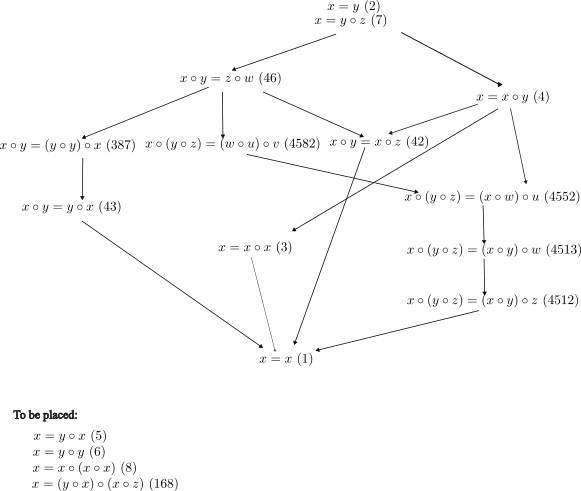
\includegraphics[width=0.5\linewidth]{../../images/implications.png}
  \caption{Implications between the above equations, displayed as a Hasse diagram.}
  \label{fig:implications}
\end{figure}


\begin{lemma}[Minimal element]\label{minimal}\uses{pre-order}  The law $0  \formaleq  0$ is the minimal element in this pre-order.
\end{lemma}

\begin{proof} Trivial.
\end{proof}

\begin{lemma}[Maximal element]\label{maximal}\uses{pre-order}  The law $0  \formaleq  0$ is the minimal element in this pre-order.
\end{lemma}

\begin{proof} Trivial.
\end{proof}

Every magma $G$ has a \emph{reversal} $G^{\mathrm{op}}$, formed by by replacing the magma operation $\circ$ with its opposite $\circ^{\mathrm{op}}:(x,y) \mapsto y \circ x$. There is a natural isomorphism between these magmas, which induces an involution $w \mapsto w^{\mathrm{op}}$ on words $w \in M_X$.  Every law $w  \formaleq  w'$ then has a \emph{dual} $w^{\mathrm{op}}  \formaleq  (w')^{\mathrm{op}}$.

For instance, the dual of the law $0 \circ 1 = 0 \circ 2$ is $1 \circ 0 = 2 \circ 0$, which after relabeling is $0 \circ 1 = 2 \circ 1$.  A list of equations and their duals can be found \href{https://github.com/teorth/equational_theories/blob/main/data/dual_equations.md}{here}.  Of the 4694 equations under consideration, 84 are self-dual, leaving 2305 pairs of dual equations.

The pre-ordering on laws has a duality symmetry:

\begin{lemma}[Duality of laws]\label{duality}\uses{pre-order}  If $w  \formaleq  w'$ implies $w''  \formaleq  w'''$, then $w^{\mathrm{op}}  \formaleq  (w')^{\mathrm{op}}$ implies $w''^{\mathrm{op}}  \formaleq  (w''')^{\mathrm{op}}$.
\end{lemma}

\begin{proof} This follows from the fact that a magma $G$ satisfies a law $w  \formaleq  w'$ if and only if $G^{\mathrm{op}}$ satisfies $w^{\mathrm{op}}  \formaleq  (w')^{\mathrm{op}}$.
\end{proof}

Some equational laws can be ``diagonalized'':

\begin{theorem}[Diagonalization]\label{diag}  An equational law of the form
  \begin{equation}\label{prediag} F(x_1,\dots,x_n) = G(y_1,\dots,y_m),
  \end{equation}
  where $x_1,\dots,x_n$ and $y_1,\dots,y_m$ are distinct elements of the alphabet, implies the diagonalized law
$$ F(x_1,\dots,x_n) = F(x'_1,\dots,x'_n).$$
where $x'_1,\dots,x'_n$ are distinct from $x_1,\dots,x_n$
In particular, if $G(y_1,\dots,y_m)$ can be viewed as a specialization of $F(x'_1,\dots,x'_n)$, then these two laws are equivalent.
\end{theorem}

\begin{proof}  From two applications of \eqref{prediag} one has
$$ F(x_1,\dots,x_n) = G(y_1,\dots,y_m)$$
and
$$ F(x'_1,\dots,x'_n) = G(y_1,\dots,y_m)$$
whence the claim.
\end{proof}

Thus for instance, Definition \ref{eq7} is equivalent to Definition \ref{eq2}.

\begin{theorem}[Laws implied by the constant law]\label{constant-impl}\uses{impl,eq46}  If $w, w'$ each have order at least one, then the law $w \formaleq w'$ is implied by the constant law (Definition \ref{eq46}).  If exactly one of $w, w'$ has order zero, and the law $w \formaleq w'$ is not implied by the constant law.
\end{theorem}

\begin{proof} Routine.
\end{proof}

\begin{theorem}[Criterion for implication]\label{variable-impl}\uses{impl}  If $w \formaleq w'$ is such that every variable appears the same number of times in both $w$ and $w'$, and $w \formaleq w'$ implies another law $w'' \formaleq w'''$, then every variable appears the same number of times in both $w''$ and $w'''$.
\end{theorem}

\begin{proof} Consider the magma $\R$ with the addition law $+$.  By hypothesis, this magma obeys $w \formaleq w'$, and hence $w'' \formaleq w'''$, giving the claim by comparing coefficients of the linear forms associated to $w''$ and $w'''$ in this magma.
\end{proof}

\chapter{Implications between selected laws}

We collect here some notable implications between the the selected laws in Chapter \ref{subgraph-eq}.   By Theorem \ref{sound-complete}, every implication can basically be established by a finite number of rewrites.  In most cases, the sequence of rewrites is quite straightforward, and the implication is very easy, but we record some less obvious examples.

\begin{theorem}[387 implies 43]\label{387_implies_43}\uses{eq387,eq43}\lean{Subgraph.Equation387_implies_Equation43}\leanok  Definition \ref{eq387} implies Definition \ref{eq43}.
\end{theorem}

\begin{proof}\leanok (From \href{https://mathoverflow.net/a/450905/766}{MathOverflow}).
  By Definition \ref{eq387}, one has the law
\begin{equation}\label{387-again}
  (x \op x) \op y = y \op x.
\end{equation}
Specializing to $y=x \op x$, we conclude
$$(x \op x) \op (x \op x) = (x \op x) \op x$$
and hence by another application of \eqref{eq387} we see that $x \op x$ is idempotent:
\begin{equation}\label{idem}
  (x \op x) \op (x \op x) = x \op x.
\end{equation}
Now, replacing $x$ by $x \op x$ in \eqref{387-again} and then using \eqref{idem} we see that
$$ (x \op x) \op y = y \op (x \op x)$$
so in particular $x \op x$ commutes with $y \op y$:
\begin{equation}\label{op-idem} (x \op x) \op (y \op y) = (y \op y) \op (x \op x).
\end{equation}
Also, from two applications of \eqref{387-again} one has
$$(x \op x) \op (y \op y) = (y \op y) \op x = x \op y.$$
Thus \eqref{op-idem} simplifies to $x \op y = y \op x$, which is Definition \ref{eq43}.
\end{proof}

\begin{theorem}[29 equivalent to 14]\label{29_equiv_14} \uses{eq29,eq14}\lean{Subgraph.Equation29_implies_Equation14}\leanok  Definition \ref{eq29} is equivalent to Definition \ref{eq14}.
\end{theorem}

This result was posed as Problem A1 from Putnam 2001.

\begin{proof}\leanok\uses{duality} By Lemma \ref{duality} it suffices to show that Definition \ref{eq29} implies Definition \ref{eq14}.  From Definition \ref{eq29} one has
  $$ x = ((x \op y) \op x) \op (x \op y)$$
  and also
  $$ y = (x \op y) \op x$$
  giving $x = y \op (x \op y)$, which is Definition \ref{eq14}.
\end{proof}

\begin{theorem}[14 implies 29]\label{14_implies_29} \uses{eq29,eq14}\lean{Subgraph.Equation14_implies_Equation29}\leanok  Definition \ref{eq14} implies Definition \ref{eq29}.
\end{theorem}

This result was posed as Problem A1 from Putnam 2001.

\begin{proof}\leanok
\end{proof}

The following result was Problem A4 on Putnam 1978.

\begin{theorem}[3744 implies 3722, 381]\label{3744_implies_3722_381}\uses{eq3744, eq3722, eq381}\lean{Subgraph.Equation3744_implies_Equation3722, Subgraph.Equation3744_implies_Equation381}\leanok Definition \ref{eq3744} implies Definition \ref{eq3722} and Definition \ref{eq381}.
\end{theorem}

\begin{proof}\leanok By hypothesis, one has
$$x \op y = (x \op z) \op (w \op y)
  $$
for all $x,y,z,w$.  Various specializations of this give
\begin{align}
 x \op y &= (x \op z) \op (y \op y) \label{381-1} \\
 x \op z &= (x \op z) \op (x \op z) \label{381-2} \\
(x \op z) \op y &= ((x \op z) \op (x \op z)) \op (y \op y) \label{381-3}.
\end{align}
The equation \eqref{381-2} gives Definition \ref{eq3722}, while \eqref{381-1}, \eqref{381-2}, \eqref{381-3} gives
$$ x \op y = (x\op z) \op y$$
which is Definition \ref{eq381}.
\end{proof}

\begin{theorem}[1689 is equivalent to 2]\label{1689_equiv_2}\uses{eq1689, eq2}\lean{Subgraph.Equation1689_implies_Equation2, Subgraph.Equation2_implies_Equation1689}\leanok Definition \ref{eq1689} is equivalent to Definition \ref{eq2}.
\end{theorem}


\begin{proof}\leanok  The implication of Definition \ref{eq1689} from Definition \ref{eq2} is trivial.  The converse is a surprisingly long chain of implications; see pages 326--327 of \cite{Kisielewicz2}.  The initial law
$$ x = (y \op x) \op ((x \op z) \op z)$$
is used to obtain, in turn,
$$ x \op ((((x \op y) \op y) \op z) \op z) = (x \op y) \op y,$$
$$(x \op (y \op z)) \op (z \op ((z \op w) \op w)) = y \op z,$$
$$x \op (y \op ((y \op z) \op z)) = (x \op y) \op y,$$
$$((x \op (y \op z)) \op z) \op z = y \op z,$$
$$(x \op (y \op (z \op w))) \op (z \op w) = y \op (z \op w),$$
$$(x \op (y \op z)) \op (y \op z) = x \op (y \op z),$$
$$((x \op y) \op ((y \op z) \op z)) \op ((y \op z) \op z) = y,$$
$$((x \op y) \op ((y \op z) \op z)) \op ((y \op z) \op z) = ((x \op ((x \op y) \op ((y \op z) \op z))) \op ((y \op z) \op z)) \op ((y \op z) \op z),$$
$$ x \op ((x \op y) \op y) = x,$$
$$ x \op (x \op (y \op z)) = x,$$
$$ (x \op y) \op y = x \op y,$$
$$ (x \op x) \op x = x,$$
$$ (x \op y) \op y = y,$$
$$ x \op y = y.$$
\end{proof}

The following result was established in \cite{mendelsohn-padmanabhan}.

\begin{theorem}[Consequences of 1571]\label{1571_impl}\uses{eq1571, eq2662, eq40, eq23, eq8, eq16, eq14, eq43, eq4512}\lean{Subgraph.Equation1571_implies_Equation2662, Subgraph.Equation1571_implies_Equation40, Subgraph.Equation1571_implies_Equation23,Subgraph.Equation1571_implies_Equation8, Subgraph.Equation1571_implies_Equation16, Subgraph.Equation1571_implies_Equation43, Subgraph.Equation1571_implies_Equation4512}\leanok  Magmas obeying Definition \ref{eq1571} also obey Definitions \ref{eq2662}, \ref{eq40}, \ref{eq23}, \ref{eq8}, \ref{eq16}, \eqref{eq14}, \ref{eq43}, and \ref{eq4512}, and are in fact abelian groups of exponent two.  Conversely, all abelian groups of exponent two obey Definition \ref{eq1571}.
\end{theorem}

\begin{proof}\leanok  Suppose that a magma $G$ obeys Definition \ref{eq1571}, thus
\begin{equation}\label{1571-again}
 x = (y \op z) \op (y \op (x \op z)).
\end{equation}
$$ x = ((x \op y) \op (x \op y)) \op ((x \op y) \op (x \op (x \op y)))$$
and
$$ x = (x \op y) \op (x \op (x \op y))$$
whence
$$x = ((x \op y) \op (x \op y)) \op x$$
which is Definition \ref{eq2662}.  This gives
$$y = ((y \op z) \op (y \op z)) \op y$$
while from \eqref{1571-again} one has
$$ (y \op z) \op (y \op z) = (x \op y) \op (x \op ((y \op z) \op (y \op z) \op y))$$
whence
$$ (x \op y) \op (x \op y) = (y \op z) \op (y \op z).$$
This implies that $(x \op y) \op (x \op y)$ does not depend on $x$, or on $y$, hence is equal to some constant $e$:
$$ (x \op y) \op (x \op y) = e.$$
From \eqref{1571-again} the magma operation is surjective, hence
\begin{equation}\label{xxe} x \op x = e
\end{equation}
which gives Definition \ref{eq40}.  Applying \eqref{1571-again} with $x=y=z$ we conclude
$$ x = e \op (x \op e)$$
while if we instead take $y=z=e$ we have
$$ x = e \op (e \op (x \op e))$$
hence
$$ x = e \op x$$
and then also
$$ x = x \op e$$
from which we readily conclude Definitions \ref{eq23}, \ref{eq8}; thus $e$ is an identity element.  From \eqref{1571-again} with $z=e$ we now have
\begin{equation}\label{16-again}
 x = y \op (y \op x)
\end{equation}
which is Definition \ref{eq16}. If instead we take $y=e$ we have
\begin{equation}\label{14-again}
  x = z \op (x \op z)
\end{equation}
which is Definition \ref{eq14}.  So if we substitute $z = x \op y$ and use \eqref{16-again} we obtain
$$ x = (x \op y) \op y$$
and hence
$$ y \op x = y \op ((x \op y) \op y) = x \op y$$
thanks to \eqref{14-again}.  This gives Definition \ref{eq43}, thus $G$ is now commutative.  From \eqref{1571-again} once more one has
$$x \op (y \op z) = (y \op x) \op (z \op ((x \op (y \op z)) \op x))$$
which one can simplify using commutativity and \eqref{16-again} (or \eqref{14-again}) to eventually obtain
$$x \op (y \op z) = (x \op y) \op z$$
which is Definition \ref{eq4512}.  $G$ is now commutative and associative, and every element is its own inverse and of exponent $2$, hence is an abelian group thanks to \eqref{xxe}, so $G$ is an abelian group of exponent $2$ as claimed.  The converse is easily verified.
\end{proof}

\begin{theorem}[953 is equivalent to 2]\label{953_equiv_2}\uses{eq953, eq2}\lean{Subgraph.Equation953_implies_Equation2}\leanok  Definition \ref{eq953} is equivalent to Definition \ref{eq2}.
\end{theorem}

\begin{proof}\leanok  It suffices to show that Definition \ref{eq953} implies Definition \ref{eq2}.  Pick an element $0$ of $G$ and define $1 = 0 \op 0$ and $2 = 1 \op 1$ (we do not require $0,1,2$ to be distinct).
From Definition \ref{eq953} with $x=z=0$ we have
$$ 0 = y \op 2.$$
If we then apply Definition \ref{eq953} with $z=1$ we conclude that
$$ x = y \op 0$$
for all $x,y$, from which one concludes $x=x'$ for any $x,x' \in G$, giving Definition \ref{eq2}.
\end{proof}


Some other notable equational laws are as follows.

\begin{theorem}[Sheffer stroke axiom]\label{sheffer}  The law
$$ 0 \formaleq (1 \op ((0 \op 1) \op 1)) \op (0 \op (2 \op 1))$$
or in equation form
$$ x = y \op ((x \op y) \op y) \op (x \op (z \op y)) $$
axiomatizes the Sheffer stroke operation. {\bf TODO: locate the equation number for this law.}
\end{theorem}

\begin{proof}
See \cite{mccune_et_al}.  In fact this is the shortest law with this property.
\end{proof}

A \emph{natural central groupoid} is, up to isomorphism, a magma with carrier $S \times S$ for some set $S$ and operation
$$ (a,b) \op (c,d) = (b,c).$$
These are examples of central groupoids (Definition \ref{eq168}).

\begin{theorem}[Natural central groupoid axiom]\label{natural-central-groupoid}  The law
$$ 0 \formaleq (1 \op ((2 \op 0) \op 3)) \op (0 \op 3)$$
or in equation form
\begin{equation}\label{26302}
  x = (y \op ((z \op x) \op w)) \op (x \op w)
\end{equation}
(Equation 26302) characterizes natural central groupoids.
\end{theorem}

\begin{proof}
  See \cite[Theorem 5]{knuth}.  The proof is quite lengthy; a sketch is as follows. It is easy to see that natural central groupoids obey \eqref{26302}.  Conversely, if this law holds, then
\begin{align*}
  (y \op z) \op (z \op w) &= (( x \op ((w \op (y \op z)) \op w)) \op ((y \op z) \op w)) \op (z \op w)\\
  &= z
\end{align*}
so we have a central groupoid.  Setting $y = (t \op t) \op t$, $z = t \op (t \op t)$, $w = t \op t$ in \eqref{26302} we also obtain
$$ (x \op t) \op t = (t \op t) \op t.$$
Using the notation
$$ x^{(1)} := (x \op x) \op x, \quad x^{(2)} := x \op (x \op x)$$
we then have
\begin{align*}
  x \op t &= ((x \op x) \op (x \op t)) \op ((x \op t) \op t) \\
  &= x \op t^{(1)}.
\end{align*}
A lengthy computer-assisted argument then gave the dual identity
$$ t^{(2)} \op x = t \op x$$
Together, these give
$$ x^{(2)} \op y^{(1)} = x \op y.$$
Multiplying on the left by $x = x^{(1)}\op x^{(2)}$, one can conclude that
$$ x^{(2)} = x \op (x \op y).$$
One then has
\begin{align*}
  (x \op y)^{(1)} &= ((y \op x) \op (x \op y)) \op (x \op y) \\
&= x \op (x \op y) \\
&= x^{(2)}
\end{align*}
and a similar argument gives
$$ (x \op y)^{(2)} = y^{(1)}.$$
Since $(x \op x)^{(1)} = x^{(2)}$ and $(x \op x)^{(2)} = x^{(1)}$, we conclude that $x^{(1)}$ and $x^{(2)}$ are idempotent.  Since $x = x^{(1)} \op x^{(2)}$, we see that every $x$ is the product of two idempotents.  One can show that this representation is unique, and gives a canonical identification with a natural central groupoid.
\end{proof}

\chapter{Selected magmas}

Each magma can be used to establish anti-implications: if $\Gamma$ is the set of all laws obeyed by a magma $G$, then we have $\not E \leq E'$ whenever $E \in \Gamma$ and $E' \not \in \Gamma$.  Large numbers of implications can already be obtained from

\begin{itemize}
  \item All magmas of order at most $4$, up to isomorphism (of which there are $178,985,294$);
  \item All commutative magmas of order $5$, up to isomorphism {\bf determine their count};
  \item Cyclic groups $\Z/N\Z$ with $2 \leq N \leq 12$ and $x \circ y = ax^2+bxy+cy^2+dx+ey$ for randomly chosen $a,b,c,d,e$.
  \item There are only $1410$ distinct cancellative magmas of order $5$ (up to isomorphism), and Mace4 can generate all of them in under 20 seconds. A shell script to do this is available \href{https://github.com/zaklogician/equational_theories/tree/cancellative_magmas/scripts/cancellative_magmas}{here}. A magma is cancellative if $xy=xz$ implies $y=z$ and $yx=zx$ implies $y=z$.
\end{itemize}


Some other magmas have been used to establish counterexamples:
\begin{itemize}
  \item The cyclic group $\Z/6\Z$ with the addition law.
  \item The natural numbers with law $x \circ y = x+1$.
  \item The natural numbers with law $x \circ y = xy+1$.
  \item The reals with $x \circ y = (x+y)/2$.
  \item The natural numbers with $x \circ x$ equal to $x$ when $x=y$ and $x+1$ otherwise.
\end{itemize}

\chapter{Equivalence with the constant and singleton laws}

\href{https://github.com/teorth/equational_theories/blob/main/equational_theories/Generated/Constant.lean}{85 laws}
have been shown to be equivalent to the constant law (Definition \ref{eq46}), and
\href{https://github.com/teorth/equational_theories/blob/main/equational_theories/Generated/Singleton.lean}{815 laws}
have been shown to be equivalent to the singleton law (Definition \ref{eq2}).

These are the laws up to 4 operations that follow from diagonalization of \ref{eq2} and \ref{eq46}.

To formalize these in Lean, a search was run on the list of equations to discover
diagonalizations of these two specific laws: equations of the form $x = R$ where $R$ doesn't include
$x$, and equations of the form $x \circ y = R$ where $R$ doesn't include $x$ or $y$.

The proofs themselves all look alike, and correspond exactly to the two steps described in the proof
of \ref{diag}. The Lean proofs were generated semi-manually, using search-and-replace starting from
the output of \texttt{grep} that found the diagonalized laws.

In the case of the constant law, equation \ref{eq41} ($x \circ x = y \circ z$) wasn't detected using
this method. It was added manually to the file with the existing proof from the sub-graph project.

\chapter{Metatheorems from Invariants}
For the purposes of this chapter, a \emph{theorem} is a (true) statement about particular equations, for example `(387 implies 43)' is a theorem. A \emph{metatheorem} is a general statement about implications; one can usually get many theorems from a single metatheorem. This chapter is all about generating many interesting metatheorems using a \emph{meta-metatheorem}, called the fundamental property of invariants. If all this is making your head spin, don't worry. Look at [REFERENCES] for examples of metatheorems you can probably agree are both concrete and interesting. Once you have done that, come back here and we will show you how to prove these and other metatheorems using \emph{invariants}.

\section{Invariants}
Let $E, E_1$, and $E_2$ be equations. If $E \Rightarrow E_1$ and $E_1 \Rightarrow E_2$, then $E \Rightarrow E_2$. Very trivial. Rephrasing this, we see that if $E \Rightarrow E_1$ and $E \nRightarrow E_2$, then $E_1\nRightarrow E_2$. 

Extending this idea, suppose we compute the set of all equations which are implied by $E$; we will call this set $\mathcal{Y}(E)$ (we use $\mathcal{Y}$ because this is an example of a \href{https://en.wikipedia.org/wiki/Yoneda_lemma#The_Yoneda_embedding}{Yoneda embedding}). Then $\mathcal{Y}(E)$ is upwards closed, or closed under forward implication: no equation in $\mathcal{Y}(E)$ can imply an equation not in $\mathcal{Y}(E)$. If we know $\mathcal{Y}(E)$ well, this already settles a potentially large number of implications in the negative.

While computing $\mathcal{Y}(E)$ for an arbitrary equation $E$ may seem daunting, for some nice equations we can find \emph{invariants}, which makes the task manageable. An \emph{invariant} for $E$ is some sort of data associated with expressions $w$ so that
\[
\mathcal{Y}(E) = \{w = w' \mid \text{Invariant}(w) = \text{Invariant}(w')\}
\]
If we can find an invariant which is computable for each term $w$, then we can easily describe $\mathcal{Y}(E)$. The fact that $\mathcal{Y}(E)$ is upwards closed is rephrased as follows; this is called \textbf{the fundamental property of invariants}. Remember that an invariant is a function taking expressions and outputting some data.

\begin{metametatheorem}[Fundamental property of invariants]
	Let $I$ be an invariant of $E$. If $w = w'$ implies $w'' = w'''$ and $I(w) = I(w')$ (that is, $E$ implies $w = w'$), then $I(w'') = I(w''')$.
\end{metametatheorem}

More succinctly, for an invariant $I$ of $E$ we must have
\[
(w = w' \Rightarrow w'' = w''') \implies (I(w) = I(w') \Rightarrow I(w'') = I(w''')).
\]
When using this result, we commonly take the contrapositive: if $I(w) = I(w')$ and $I(w'') \neq I(w''')$, then $w=w'$ cannot imply $w'' = w'''$. Note that the conclusion is independent of the equation $E$; all we need to know is that $I$ is an invariant.


%I am stealing the proof environment for a note - this is probably bad practice.
\begin{proof}[Note for category theorists]\leanok
	Let $\Pi$ denote the preorder of magma equations ordered by implication. If $I$ is an invariant then define
	\[
	I(w = w')\coloneqq \begin{cases}
		\texttt{true} & \text{ if }I(w) = I(w')\\
		\texttt{false} & \text{ otherwise}
	\end{cases}.
	\]
	(In programming languages we would say $I(w = w') \coloneqq I(w) == I(w')$). Let $\textbf{Bool} = \{ \texttt{true}, \texttt{false}\}$ be the poset where $\texttt{false} \leq \texttt{true}$. Then $I$ becomes a function $\Pi \to \textbf{Bool}$, and the fundamental property of invariants just says that this function is monotone, i.e. functorial. Thus for every invariant $I$ we obtain a functor $\Pi \to \textbf{Bool}$.
	
	Question 1: Does every functor $\Pi \to \textbf{Bool}$ come from an invariant?
	
	Question 2: What can we say about the category of functors $\Pi \to \textbf{Bool}$? Give a nice interpretation of natural transformations between invariants.
\end{proof}

The fundamental property of invariants is not a theorem, nor a metatheorem: it is a meta-metatheorem, in the sense that it will allow us to get a metatheorem for every invariant we find.

\subsubsection*{Example: absorption law}
Let $E$ be the equation $x \circ y = x$. Intuitively, we must have
\[
\mathcal{Y}(E) = \{w = w' \mid \text{the leftmost variable is the same for $w$ and $w'$}\}.
\]
We will talk about proving statements like this one (say in Lean) later on; take it as given for now. The invariant is clear: we define $I(w)$ to be the leftmost variable of $w$. Instantiating this invariant in the fundamental property of invariants, we get the following metatheorem.
\begin{metatheorem}
	Let $w = w'$ be an equation such that the leftmost variable of $w$ is the same as the leftmost variable of $w'$. Then $w = w'$ cannot imply an equation that does not have the property from the last sentence. 
\end{metatheorem}

\subsubsection*{Example: associativity}
For a more complicated example, let $E$ be the associativity equation $x \circ (y \circ z) = (x \circ y) \circ z$. Intuitively, we must have
\[
\mathcal{Y}(E) = \{\text{equations that, when we remove all parentheses, are of the form $w = w$}\}.
\]
There is an invariant lurking behind: it is the (ordered) list of variables appearing in an expression, counting repetitions. More formally, we define $I(w)$ to be the tuple of variables appearing in $w$, listed from left to right, say. Again, from the fundamental property of invariants we get the following.
\begin{metatheorem}
	Let $w = w'$ be an equation such that the variables appearing in $w$, taking into account order and repetitions, are the same ones that appear in $w'$. Then $w = w'$ cannot imply an equation that does not have the property from the last sentence. 
\end{metatheorem}

If we were coding a computer program that computes $I(w)$ given $w$, one could take the string of symbols that is $w$, ignore all parentheses, replace all symbols $\circ$ by commas, and surround with an appropriate delimiter. (I imagine one could easily do this using \href{https://en.wikipedia.org/wiki/Regular_expression}{regular expressions}.

We can compute other examples, but the invariant can get complicated even for simple equations. Exercise: what is the invariant for commutativity? Answer: To compute $I(w)$ from $w$ replace all parentheses with curly braces and all symbols $\circ$ with commas, and interpret the result as nested sets.

\section{Expanding the language}
The method of invariants really shines when we expand our formal language. Right now our language consists of variables, parentheses, the equal sign, and $\circ$ (there is also an implicit use of $\forall$ but let's ignore that for now).  Let $\Pi$ denote the preorder of equations (built from the language described) ordered by implication.

We will add the symbol $\wedge$ (`and') to our language. Then we consider a bigger preorder $\Pi' \supseteq \Pi$ which includes equations and also conjunctions of equations. Even if we only care about $\Pi$ it will be apparent that studying invariants in $\Pi'$ gives us useful metatheorems about $\Pi$. Equations and conjunctions of equations are examples of \emph{formulas} (or formulae, according to taste).

If $\varphi$ is a formula, we can define $\mathcal{Y}(\varphi)$ to be the set of all formulae implied by $\varphi$; this agrees with our previous definition. Now define an invariant of $\varphi$ to be a function $I$ on terms such that
\[
\mathcal{Y}(\varphi) \cap \Pi = \{w = w' \mid I(w) = I(w')\}.
\]
Again, this clearly agrees with our previous definition. Although $\mathcal{Y}(\varphi) \cap \Pi$ might not be upwards closed in $\Pi'$, it is upwards closed in $\Pi$, which is enough to get the fundamental property of invariants \emph{verbatim}. This leads to more metatheorems we didn't have access to before. 

\subsubsection*{Example: associativity and idempotency}
Let $\varphi$ be the conjunction of the associative law and the idempotency law ($x \circ x = x$). Again, we will rely on our intuition, which says that an invariant $I$ defined by taking $I(w)$ to be the set of all variables appearing in $w$, works. The corresponding metatheorem is the following

\begin{metatheorem}
	Let $w = w'$ be an equation such that the set of variables appearing in $w$ is equal to the set of variables appearing on $w'$. Then $w = w'$ cannot imply an equation that does not have the property from the last sentence. 
\end{metatheorem} 

\subsubsection*{Example: associativity and commutativity}
For a similar example, we can let $\varphi$ be the conjunction of the associative and the commutative laws. Here we can define $I(w)$ to be the \href{https://en.wikipedia.org/wiki/Multiset}{multiset} of variables appearing in $w$. We obtain the following metatheorem.

\begin{metatheorem}
	Let $w = w'$ be an equation such that the variables appearing in $w$, taking into account multiplicity, are the same ones that appear in $w'$. Then $w = w'$ cannot imply an equation that does not have the property from the last sentence. 
\end{metatheorem}

Trivia: this was the first example of a metatheorem obtained by use of an invariant.

\subsubsection*{Example: associativity and commutativity with a twist}
We can keep expanding our language if it helps us express more intricate invariants. For instance, we can add the symbol `1' to our language. Let $\varphi$ be the conjunction of associativity, commutativity, the equations $1 \circ x = x$, and
\[
\underbrace{x \circ x \circ \cdots \circ x}_{m\text{ times}} = 1,
\]
for some fixed positive integer $m$. Pause to guess the invariant before we move on.

The invariant $I(w)$ is the multiset of variables appearing in $w$ but multiplicities are computed modulo $m$. Thus we have the pretty metatheorem:
\begin{metatheorem}
	Fix some positive integer $m$. Let $w = w'$ be an equation such that every variable appearing in $w$ appears the same number of times in $w'$ modulo $m$. Then $w = w'$ cannot imply an equation that does not have the property from the last sentence. 
\end{metatheorem}

\section{Proving metatheorems from invariants in Lean}

For the rest of this chapter we readopt the convention of calling `theorem' an important result, not necessarily pertaining to specific equations.

An invariant is generally a \emph{syntactic} property of an expression. However, invariants can also be described and calculated \emph{semantically} through the notion of a \emph{lifting magma family}, described below. The general idea is that the value of an invariant for an expression can be computed by substituting specific values for the variables in the expression and evaluating the result in a certain magma in the lifting magma family; additional requirements ensure that the fundamental property of invariants is satisfied. 

\begin{definition}[Lifting Magma Family]\label{lifting-magma-family}
	A \emph{lifting magma family} is a family of magmas $\{G_\alpha\}$, one for each type $\alpha$, satisfying the following properties:
	\begin{itemize}
		\item For each type $\alpha$, there is a function $\iota_\alpha : \alpha \to G_\alpha$.
		\item Given a function $f : \alpha \to G_\alpha$, there is a magma homomorphism $\operatorname{lift}{f} : G_\alpha \to G_\alpha$ such that $\operatorname{lift}{f}(\iota_\alpha(x)) = f(x)$ for all $x$ in $\alpha$.
	\end{itemize}
\end{definition}

\begin{example}
	The free Abelian groups form a lifting magma family. When the underlying set is finite, the groups are isomorphic to $\mathbb{Z}^n$.
\end{example}

\begin{example}
	Lists form a lifting magma family.
\end{example}

The key consequence of the definition \ref{lifting-magma-family} is that it is significantly easier to check whether an equation is satisfied in a lifting magma family.

\begin{theorem}[Evaluation theorem for lifting magma families]\label{lifting-magma-basis-evaluation}
	Suppose $E$ is an equation involving a set of variables $X$, and let $G$ be a lifting magma family.
	
	Determining whether $E$ is satisfied by $G_X$ is equivalent to checking that $E$ is true with the specific substitution $\iota_X$.
	
\end{theorem}
\begin{proof}
	For the forward direction, suppose $E$ is satisfied by $G_X$. Then, by definition, any substitution of the variables in $E$ with elements of $G_X$ will yield a true equation. In particular, substituting according to $\iota_X$ will yield a true equation.
	
	For the reverse direction, suppose that $E$ is true when evaluated with the substitution $\iota_X$. Now, consider an arbitrary substitution of variables $f : X \to G_X$. By the lifting magma family property, there is a magma homomorphism $\operatorname{lift}{f} : G_X \to G_X$ such that $\operatorname{lift}{f}(\iota_X(x)) = f(x)$ for all $x$ in $X$. In other words, applying the substitution $f$ is equivalent to first applying to substitution $\iota_X$ and then applying the homomorphism $\operatorname{lift}{f}$. Since $E$ is true when evaluated with the substitution $\iota_X$, it is also true after applying the homomorphism $\operatorname{lift}{f}$. Thus, $E$ is satisfied by $G_X$.
\end{proof}

\begin{theorem}[The fundamental property of invariants]\label{fundamental-property-of-invariants}
	Let $E$ and $E'$ be equations involving a set of variables $X$, and let $G$ be a lifting magma family.
	
	If $E$ is true with the substitution $\iota_X$, and $E$ implies $E'$, then so is $E'$.
\end{theorem}
\begin{proof}
	Applying the evaluation theorem \ref{lifting-magma-basis-evaluation}, we see that $E$ is satisfied by $G_X$. Since $E$ implies $E'$, $E'$ is also satisfied by $G_X$, and in particular, $E'$ is true with the substitution $\iota_X$.
\end{proof}

\begin{remark}
	The result of evaluating an expression along the function $\iota_X : X \to G_X$ \emph{is} the invariant.
	
	In the case of Abelian groups, the result of evaluation is the variables in the expression with multiplicity.
	In the case of lists, the result of evaluation is the variables in the expression in the order they appear.
	
	When the lifting magma family has good computational properties, calculating the invariant becomes easy.
\end{remark}

\begin{remark}
	Given an equation $\phi$ in the language of magmas (possibly involving logical operations other than equality and universal quantification), the initial (i.e., most general) magmas satisfying $\phi$ (provided they exist) form a lifting magma family.
	
	However, for the purpose of generating invariants, we are interested in lifting magma families with convenient descriptions that are computationally tractable.
\end{remark}

\begin{remark}
	Suppose $S$ is a finite set of equations in the language of magmas that is a confluent term rewriting system under a certain ordering of the terms (in the sense of the Knuth-Bendix algorithm). Then the initial magmas satisfying $S$ form a lifting magma family where equality of elements in the magma is decidable.
	
	This offers a way of generating examples of lifting magma families with good compuational properties for computing invariants of expressions.
\end{remark}


\section{Conclusion: Beyond Invariants}
We are still lacking:
\begin{itemize}
	\item A large collection of invariants.
	\item An estimate for how many implications the resulting metatheorems will settle. 
	\item Algorithms (in Lean, Python, or otherwise) to compute known invariants.
	\item General results about lifting magmas.
	\item Formalization of the method of invariants and resulting metatheorems.
	\item Knowledge about the category-theoretic interpretation of invariants (see the questions in the note for category theorists).
\end{itemize}

Related to the last bullet point, we note the following. If all that matters about invariants is the fundamental property, we can apply the old French trick of turning a (meta-meta)theorem into a definition. 

Q: If we were to define invariants as any functions satisfying the fundamental property, would anything change? (For those who read the note for category theorists: an equivalent redefinition is to consider invariants as functors $\Pi \to \textbf{Bool}$).
\chapter{Simple rewrites}

\href{https://github.com/teorth/equational_theories/tree/main/equational_theories/SimpleRewrites/theorems}{53,905 implications} were automatically generated by simple rewrites.

{\bf describe the process of automatically generating these implications here.}

\chapter{Trivial auto-generated theorems}

\href{https://github.com/teorth/equational_theories/tree/main/equational_theories/Generated/TrivialBruteforce}{Approximately 4.5m transitive implications were proven by a transitive reduction of about 15k theorems}. Most of these implications were derived from being the first automated run to connect the largest equivalence classes, hence creating a large set of transitively closed implications.

Scripts generated theorems to try simple combinations of equation rewrites to reach the desired goal for every unknown implication. The generated proof scripts were run with lean and the successful theorems were extracted. An example of the types of generated rewrites that were tested:

\begin{verbatim}
  repeat intro
  apply
\end{verbatim}

\begin{verbatim}
  repeat intro
  try { rw [<-h] }
  try { rw [<-h, <-h] }
  try { rw [<-h, <-h, <-h] }
  try { rw [<-h, <-h, <-h, <-h] }
  try { rw [<-h, <-h, <-h, <-h, <-h] }
  repeat rw [h]
\end{verbatim}

\begin{verbatim}
  repeat intro
  try {
    nth_rewrite 1 [h]
    try { rw [h] }
    try { rw [<-h] }
  }
  try {
    nth_rewrite 2 [h]
    try { rw [h] }
    try { rw [<-h] }
  }
  try {
    nth_rewrite 3 [h]
    try { rw [h] }
    try { rw [<-h] }
  }
  try {
    nth_rewrite 4 [h]
    try { rw [h] }
    try { rw [<-h] }
  }
  try {
    nth_rewrite 1 [h]
    nth_rewrite 1 [h]
    try { rw [h] }
    try { rw [<-h] }
  }
  ...
\end{verbatim}

\chapter{Enumerating Small Finite Magmas}\label{all-small-magmas-chapter}

{\bf describe the process of automatically generating these implications here.}

\chapter{Equation Search}\label{equation-search-chapter}

\href{https://github.com/teorth/equational_theories/tree/main/equational_theories/Generated/EquationSearch}{Approximately ~650k transitive implications were proven by a custom tool leveraging the implication graph}. After previous brute force had derived many implications expressible as a small number of rewrites, this search tool uses substitutions implied by the implication graph to search further.

An example proof illustrates the logic it uses:

\begin{verbatim}
  have eq3315 (x y : G) : x * y = x * (y * (x * x)) := by
    apply Apply.Equation12_implies_Equation11 at h
    apply RewriteHypothesis.Equation11_implies_Equation3323 at h
    apply Apply.Equation3323_implies_Equation3315 at h
    apply h
  have eq52 (x y : G) : x = x * (y * (x * x)) := by
    apply Apply.Equation12_implies_Equation61 at h
    apply Apply.Equation61_implies_Equation54 at h
    apply Apply.Equation54_implies_Equation52 at h
    apply h
  repeat intro
  nth_rewrite 1 [eq3315]
  nth_rewrite 1 [← eq52]
  apply h
  repeat assumption
\end{verbatim}

Using the graph of implications and refutations, it identifies equivalence classes/strongly-connected components in the implication graph and possible goals by subtracting out the refutation graph. Iterating through all equivalence classes, it can perform a meet-in-the-middle graph search where it searches outwards from both hypotheses and goals by performing equation substitutions. Depending on the number of hypotheses versus goals, it dynamically adjusts the search depth on both sides based on a configured branching factor.

Due to it's naive implementation, it may only be able to perform certain substitutions in a round-about way and the graph size explodes faster than it must, so it's limited to fairly shallow search depths. Also, the tool may emit proofs without some information Lean may require, so some generated proofs have to be fixed-up afterwards.

\chapter{E-Graphs}\label{egraphs-chapter}

For proving implications, we used another technique called equality saturation~\cite{DBLP:journals/pacmpl/WillseyNWFTP21} with the \texttt{lean-egg} tactic, to automatically construct proofs.

A similar approach is being pursued in the MagmaEgg tool as well, which is a standalone program that only supports magma equalities, while the lean-egg tactic supports any Lean expression.

\section{lean-egg}

\subsection{Methodology}

The basic methodology of equality saturation is based on E-Graphs, a data structure that can store equivalence classes of terms efficiently.
We used the \texttt{lean-egg} tactic (\url{https://github.com/marcusrossel/lean-egg}), based on equality saturation as a tactic, which (re)constructs a proof from the E-graph~\cite{DBLP:journals/pacmpl/KoehlerGBGTS24} in Lean.
This means that we do not have to trust either the egg tool nor the tactic: if something goes wrong, Lean will not accept the constructed proof. In fact, we found issues with the proof reconstruction from the examples in this project.

The \texttt{lean-egg} tactic works for equational reasoning, i.e. proving equalities as consequences of other equalities (potentially universally quantified), which is exactly what we need to prove implications of laws in Magmas.
In many cases, we have laws of the form $x = y$, where neither set of variables in the left- and right-hand-side of the law is a subset of each other.
In this case the laws cannot be used as rewrite rules: it's not clear what it would be rewritten to, since there are unknowns on both sides of the equation.
For these cases we used a simple heuristic, where we instantiate the variables with terms found in the (proof) context, as those are likely to be important for proving the equality.

\subsection{Results}

Out of the possible implications between the $34$ equations considered in \Cref{subgraph-eq}, this method found an additional 86 implications that were not found before.
Some of these seem to be missing in the computation of the transitive closure of implications of the equalities (an investigation is in progress), but some of these are genuinely new theorems, and the \texttt{lean-egg} tactic finds good proofs of these (these can be rewritten using \texttt{calc} style with a different tactic, \texttt{calcify}: \url{https://github.com/nomeata/lean-calcify}). An example of this is the following proof, found by \texttt{lean-egg}:

\begin{theorem}[14 implies 23]\label{14_implies_23} \uses{eq23,eq14}\lean{Subgraph.Equation14_implies_Equation23}\leanok  \Cref{eq14} is equivalent to \Cref{eq23}.
\end{theorem}

\begin{proof}\leanok

$$ x = (x \op x) \op (x \op (x \op x)) = (x \op x) \op x $$
\end{proof}

It was also able to (re)prove \Cref{1689_equiv_2}, albeit with a manually-provided hint (guide, in the sense of~\cite{DBLP:journals/pacmpl/KoehlerGBGTS24}).

\section{MagmaEgg}

This is a simple but apparently at least somewhat effective Rust theorem prover based on egg \texttt{e-graph} library written for this project.

It proved $5574$ of the $24283$ implications in the \texttt{only\_strongest.txt} file at the time.

The code was originally based on the \texttt{magma\_search} pull request, but has been pretty much completely rewritten.

Currently search just uses the egg library in a basic fashion, except that in case there are extra variables not present in the LHS, it has code to instantiate them with all subexpressions of the original goal.

Exporting the proofs to Lean has turned out to be harder than finding the proofs, but a good solution has been implemented (modulo some issues in egg that require to sometimes turn off explanation optimization since it sometimes triggers stack overflows and assert failures) that directly produces proof terms using \texttt{let} / \texttt{have} and \texttt{Eq.refl}, \texttt{Eq.symm}, \texttt{Eq.trans}, \texttt{Magma.op}, a congruence lemma for \texttt{Magma.op} and variables and the hypothesis. I define one letter aliases for them to reduce verbosity.

Possible future work:

\begin{itemize}
	\item Figure out which implications are important to prove and try it on them
	\item Replace the fork-based code with self-execution so that it works on Windows and is less of na hack
	\item Fork egg and fix the buggy and slow length optimization of explanations
	\item Maybe write Lean code directly instead of writing explanation sexps and converting to Lean code in a second run
	\item Fix the generation of extra variable values so it doesn't take too much time in pathological cases (i.e. goals with 4-6 variables)
	\item Determine whether it actually has some advantages compared to Vampire and \texttt{lean-egg}
	\item Support searching for multiple goal equations at once
	\item Write a custom elaborator for Lean to speed up elaboration
	\item If the Lean kernel turns out to be too slow for some large necessary proofs and thus the custom elaborator is not enough, write a custom verified typechecker
	\item Support having extra rewrite rules, such as other implications that have been found implied by the hypothesis, or simple equalities found by the egraph search itself
	\item Run it with massive computing resources if deemed useful and someone offers those, once it's a bit more mature
\end{itemize}


\bibliographystyle{plain} % We choose the "plain" reference style
\bibliography{references}

\end{document}
